\chapter{{\bf Theory of }\boldmath{$B\to \mu^+ \mu^-$}{\bf decays; the Standard Model and beyond}}
\label{sec:theory_chptr}
This chapter describes the theoretical motivation for the study of \bmumu decays. 
In the SM these decays are predicted to occur very rarely; Section~\ref{sec:bsmumu_in_SM} describes why \bmumu decays are suppressed compared to other decay modes of \bsd mesons in the SM. The \BF of \bmumu decays provides a good observable to compare experimental measurements with predictions of the SM. The determination of the theoretical predictions of \BFs is outlined in Section~\ref{sec:BFdef} and the discussion is based on references~\cite{Blake:2016olu,Anikeev:2001rk}.
%The description of these decays within the SM framework is presented in Section~\ref{sec:bsmumu_in_SM} and the determination of the theoretical predictions of \BFs is outlined in Section~\ref{sec:BFdef}.
%The discussion of the theoretical \BFs is based on references~\cite{Blake:2016olu,Anikeev:2001rk}. 
Quark mixing leads to oscillations between \bs and \barbs states over time and therefore a difference between the values of the predicted and measured \bsmumu \BFs. These oscillations and the influence on the \BFs values are described in Section~\ref{sec:quarkmaixing} and follows the material in references~\cite{ Anikeev:2001rk,Dunietz:2000cr,Nierste:2009wg}. 
A parameter, \ADG, arises from the difference between \bs and \barbs mesons, this observable is complementary to the \BF of \bsmumu decays in the study of the SM and it can be measured through the effective lifetime of \bsmumu decays as described in Section~\ref{sec:ADG_EL}. The SM predictions for \bmumu \BFs and the \bsmumu effective lifetime are given in Section~\ref{sec:SM_predictions} and the ways in which NP can influence these observables is briefly discussed in Section~\ref{sec:NPmodels}.



\section[$B^0_{(s)}\to \mu^+ \mu^-$ decays in the Standard Model]{\boldmath{$B^0_{(s)}\to \mu^+ \mu^-$} decays in the Standard Model}
\label{sec:bsmumu_in_SM}
%Prehaps I should mention anti-particles earlier?
In the SM, quarks and anti-quarks can be combined in pairs to form mesons that are held together by the strong force. The neutral $B$ mesons, \bd and \bs, consist of a $\bar{b}$ quark combined with a $d$ quark for the \bd and an $s$ quark for the \bs. Their anti-particles, \barbd and \barbs, are formed by swapping over which quark in the pair is the anti-quark. These particles are unstable and exist for $\sim10^{-12}$~s before decaying into leptons, lighter mesons or a combination of both. One decay mode is when the \bsd decays into two oppositely charged muons as \bmumu. %~\footnote{\bmumu refers to both the particle and anti-particle decays of the \bd and \bs unless otherwise specified.}. This decay mode occurs very rarely in the SM compared to other decay modes of the \bsd. The suppression of this mode arises from several different sources.
These decay modes occur very rarely in the SM compared to other decays modes of the \bsd. The fraction of \bd and \bs mesons that decay into two muons is $\sim10^{-10}$ and $\sim10^{-9}$, respectively. The suppression of \bmumu decays comes from three sources that are described in the following.


The first source of suppression is due to the quarks that form the \bd and \bs mesons. The composite quarks of a \bsd both have the same charge magnitude, therefore in the decay \bmumu only quark flavour and not quark charge changes. This type of decay is called a flavour changing neutral current (FCNC). These decays must proceed via the weak force because it is the only interaction in which quark flavour is not conserved via the exchange of a $W$ boson. However, FCNCs are forbidden in the SM to occur at the tree level by the GIM mechanism~\cite{PhysRevD.2.1285}. Therefore \bmumu decays proceed via more complex diagrams such as $W$-box and $Z^0$-penguin diagrams as shown in Figure~\ref{fig:SM_diag}.
The decays can also proceed via Higgs-penguin diagrams however the contributions from these diagrams are negligible~\cite{Arbey:2012ax}. %within the SM. 
The lack of \bmumu decays at the tree level causes them to be suppressed compared to other \bsd decay modes that can occur at the tree level.

\begin{figure}[bt]
    \centering
        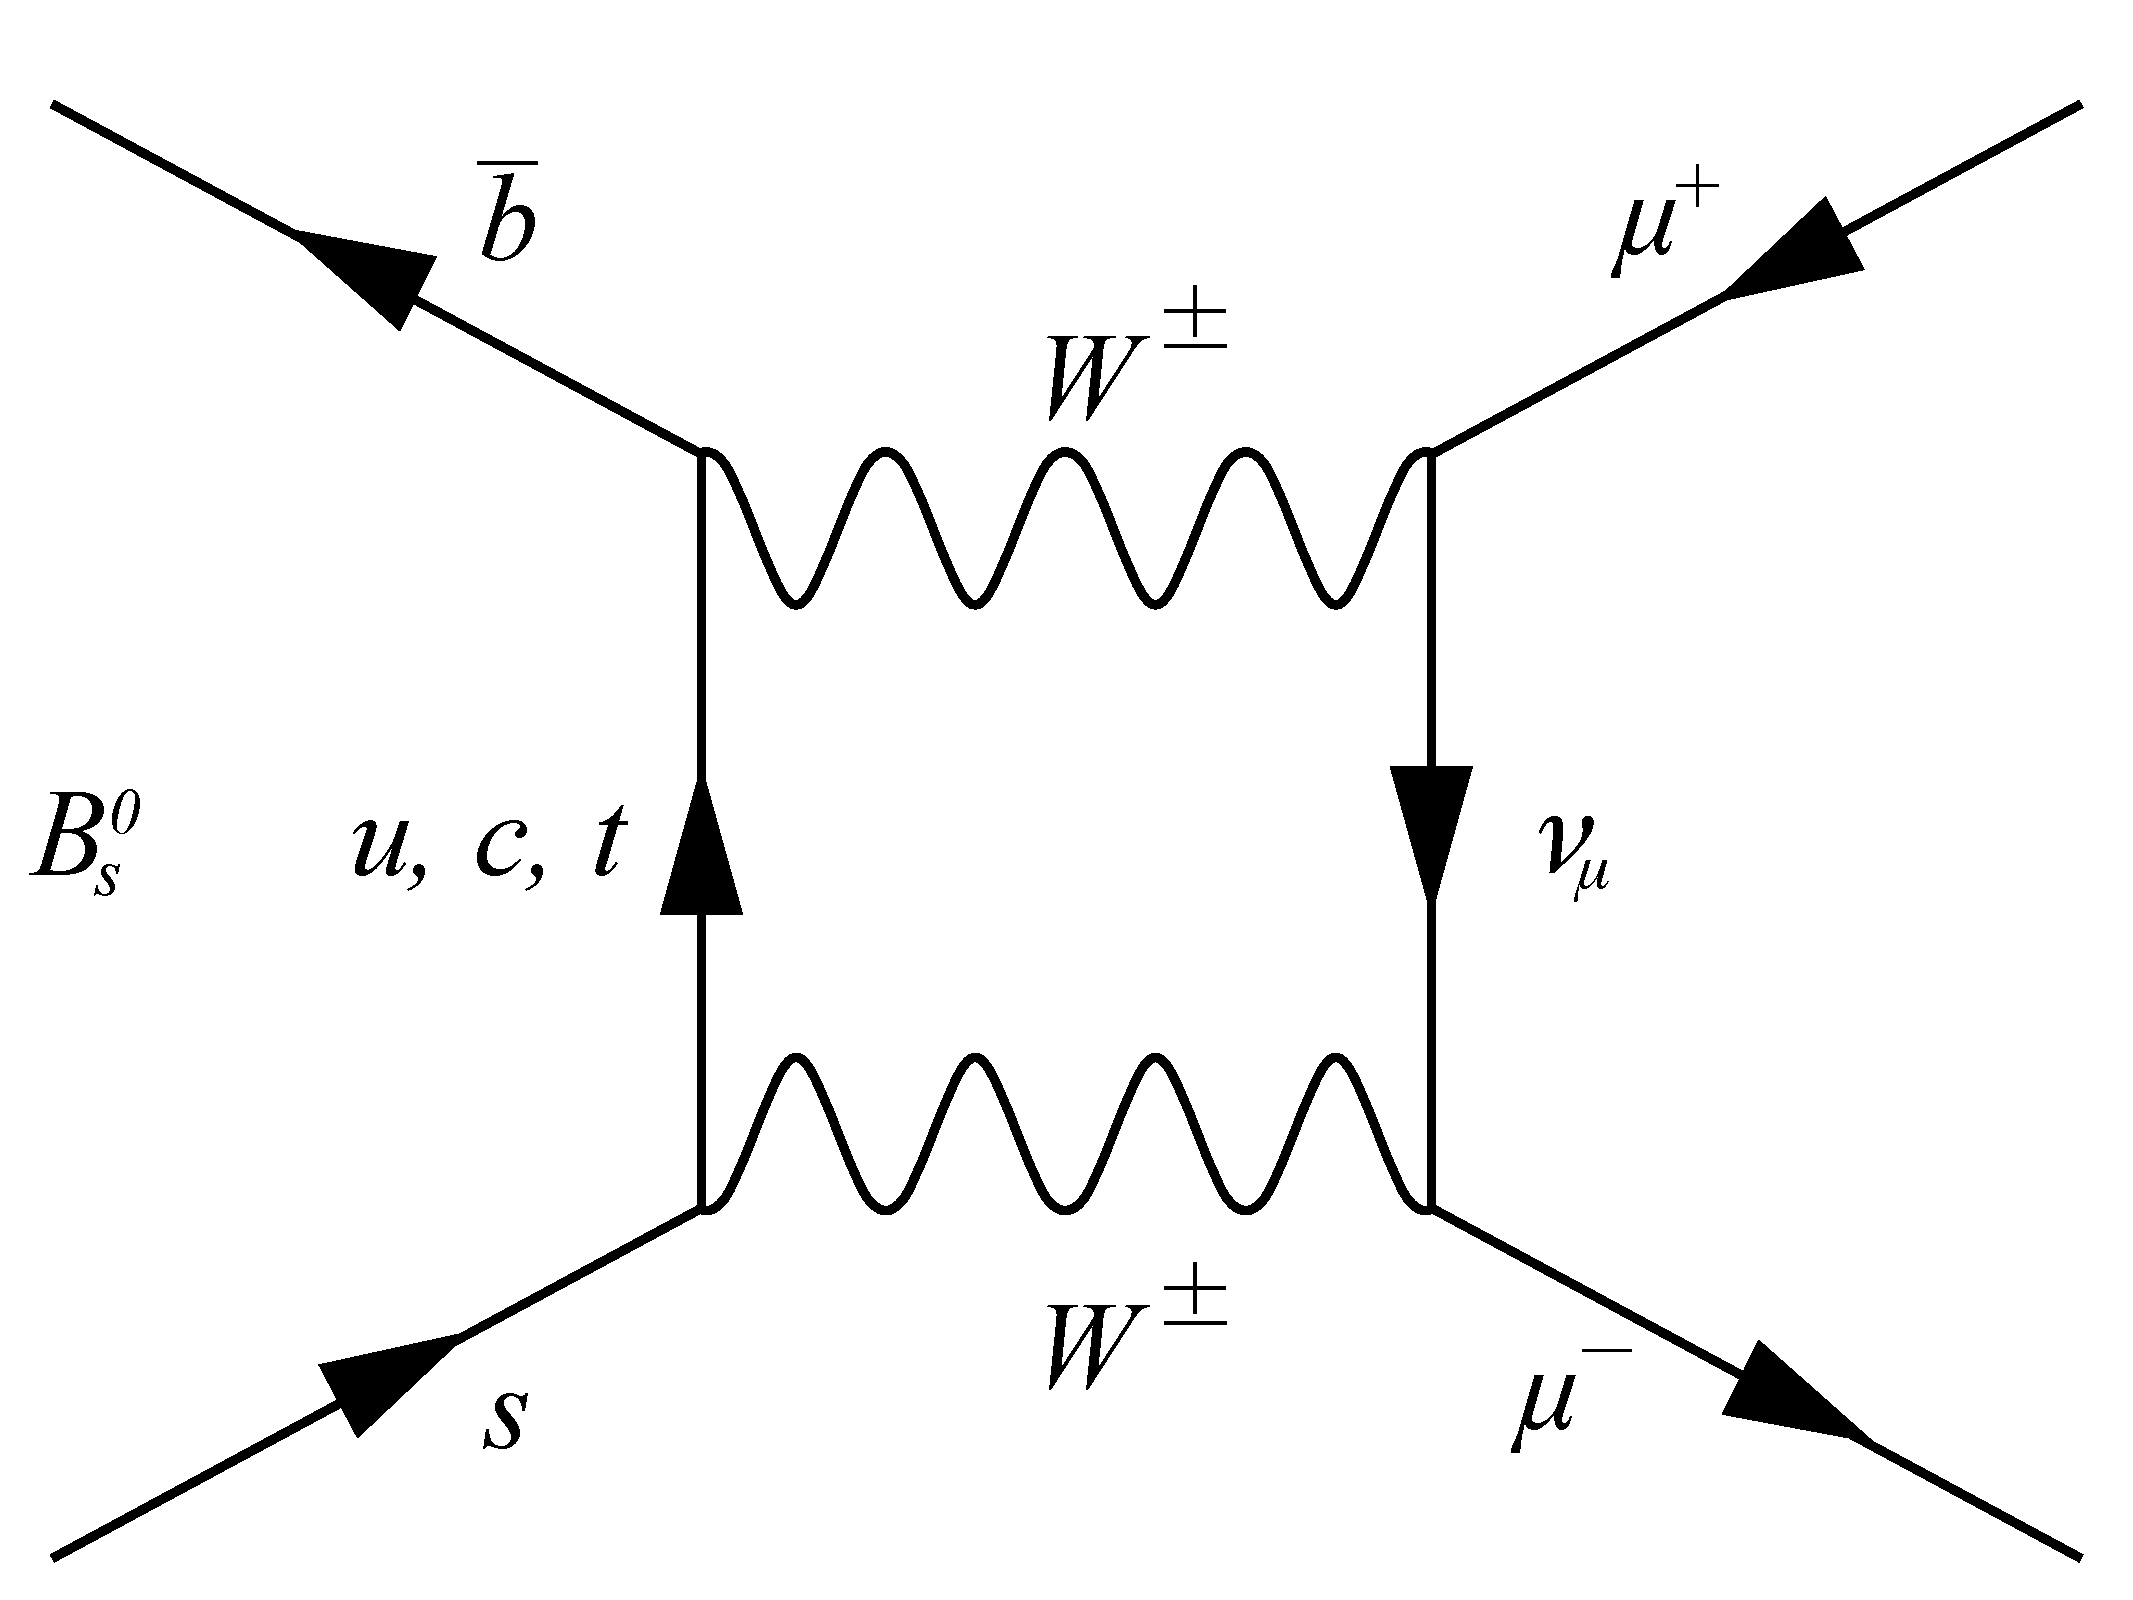
\includegraphics[width=0.4\textwidth]{./Figs/Theory/W_diagram_2.pdf}
        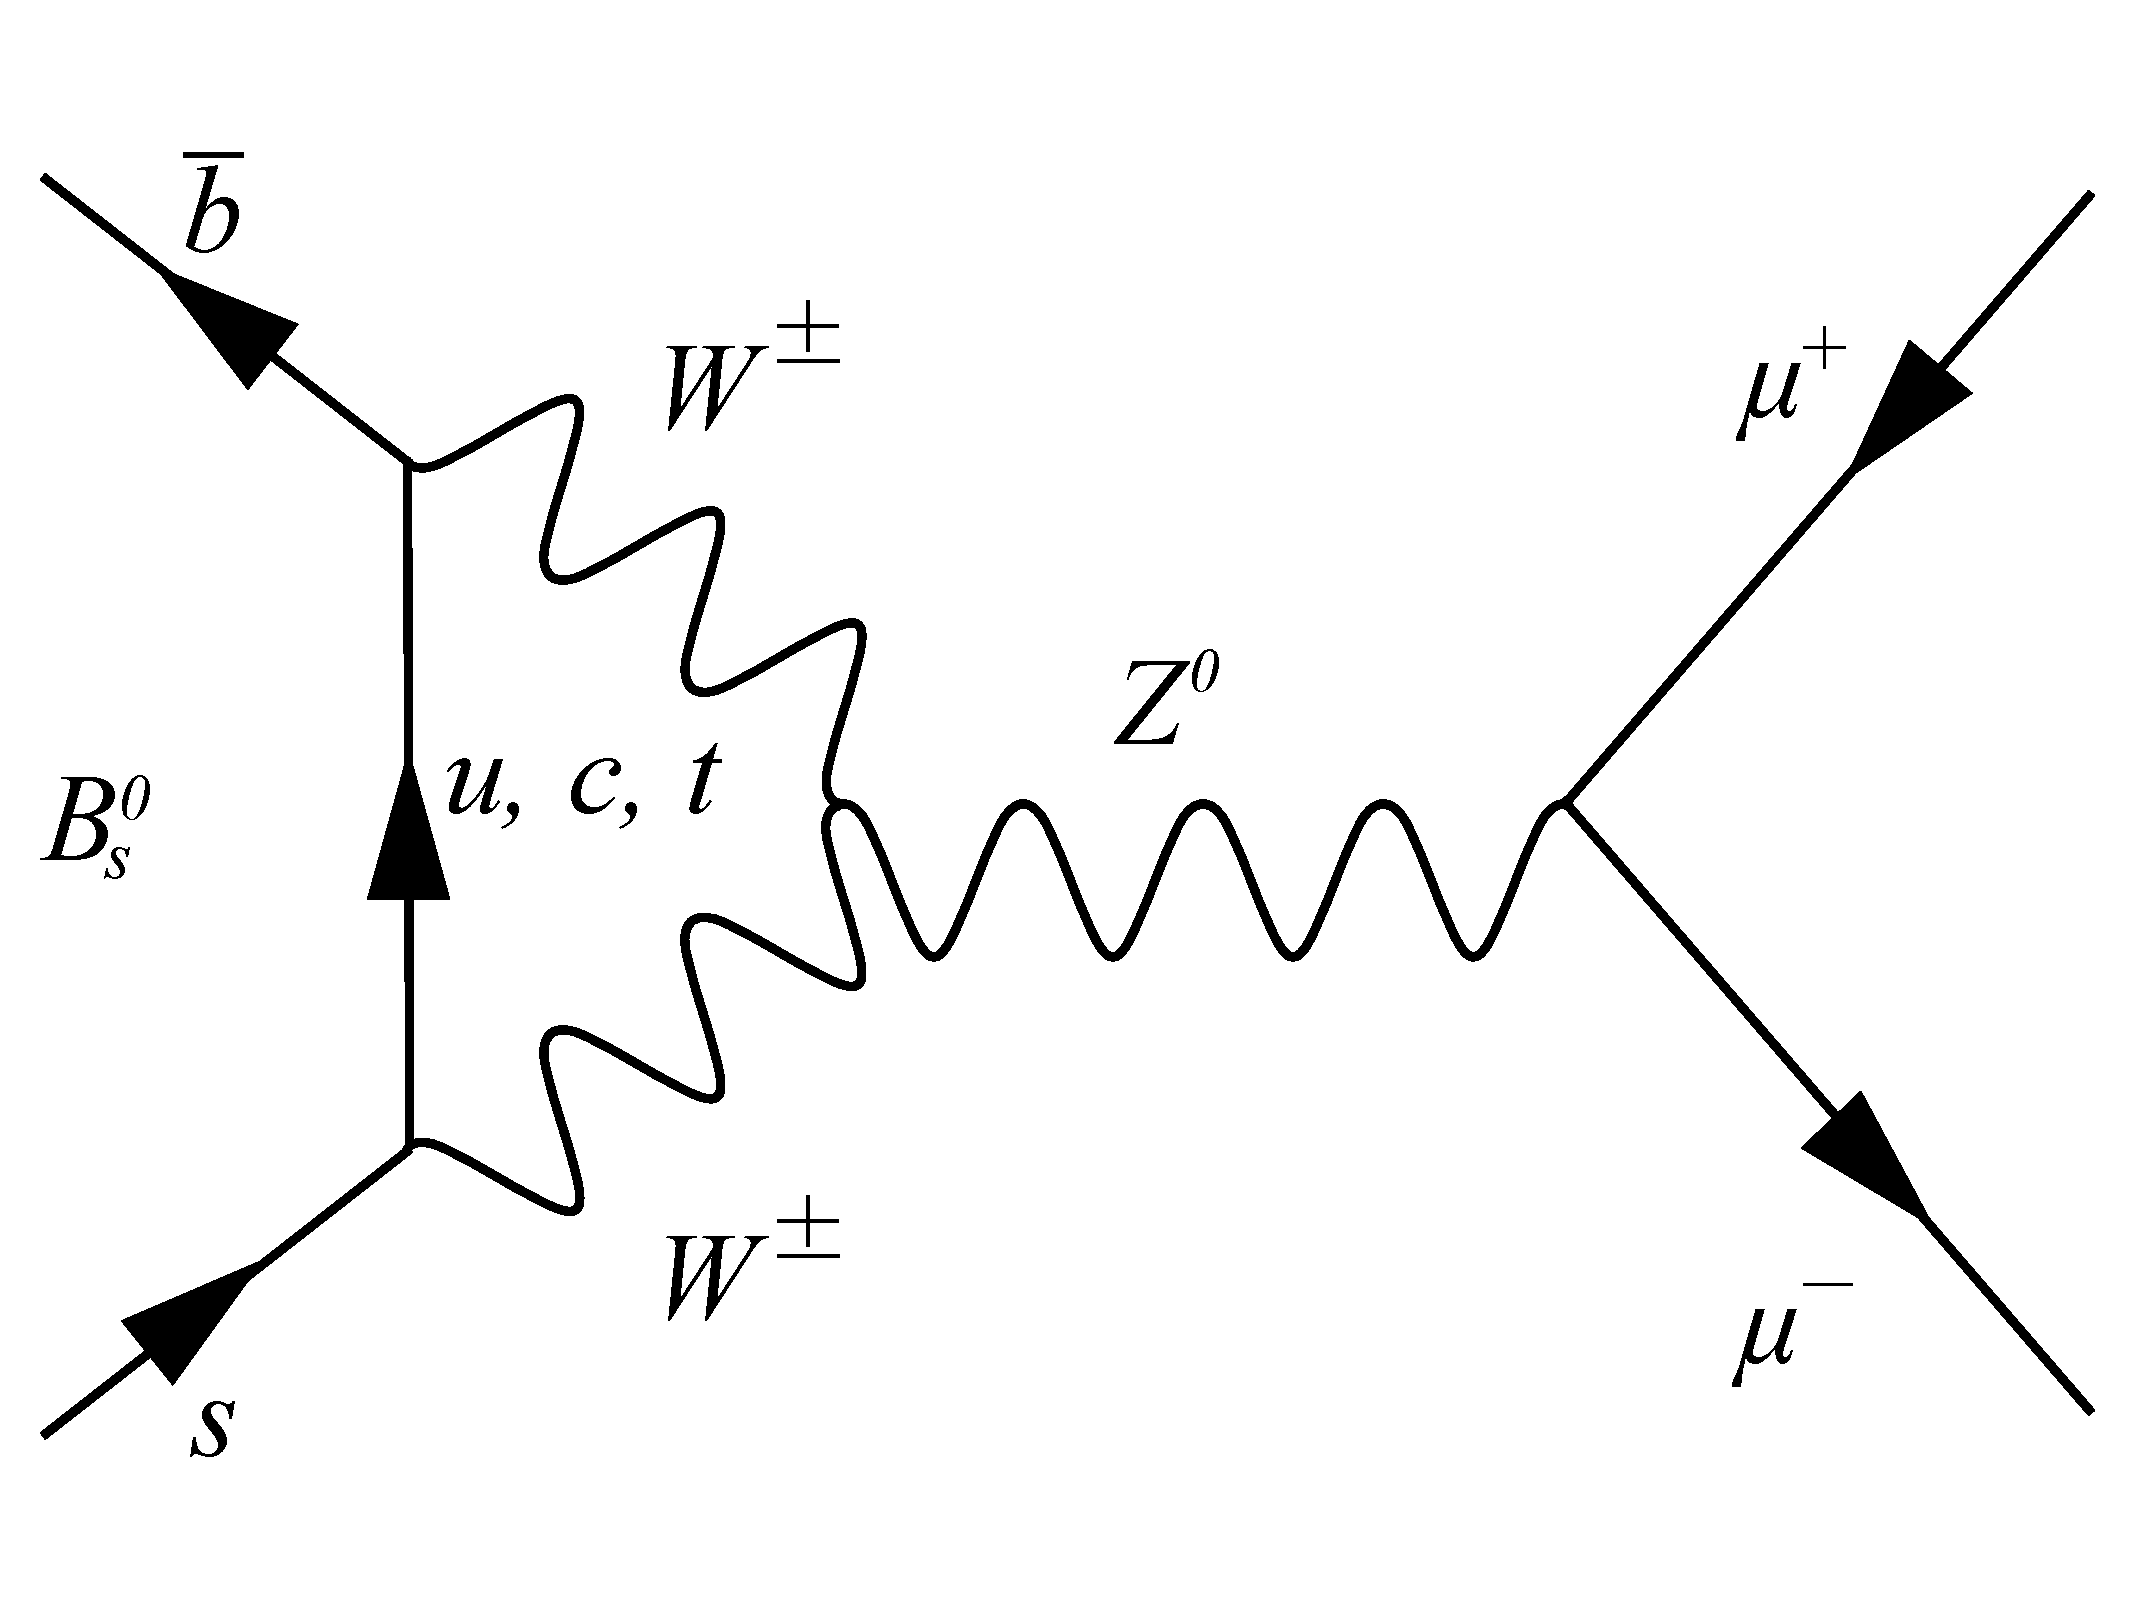
\includegraphics[width=0.4\textwidth]{./Figs/Theory/Z0_penguin_v1.pdf}
        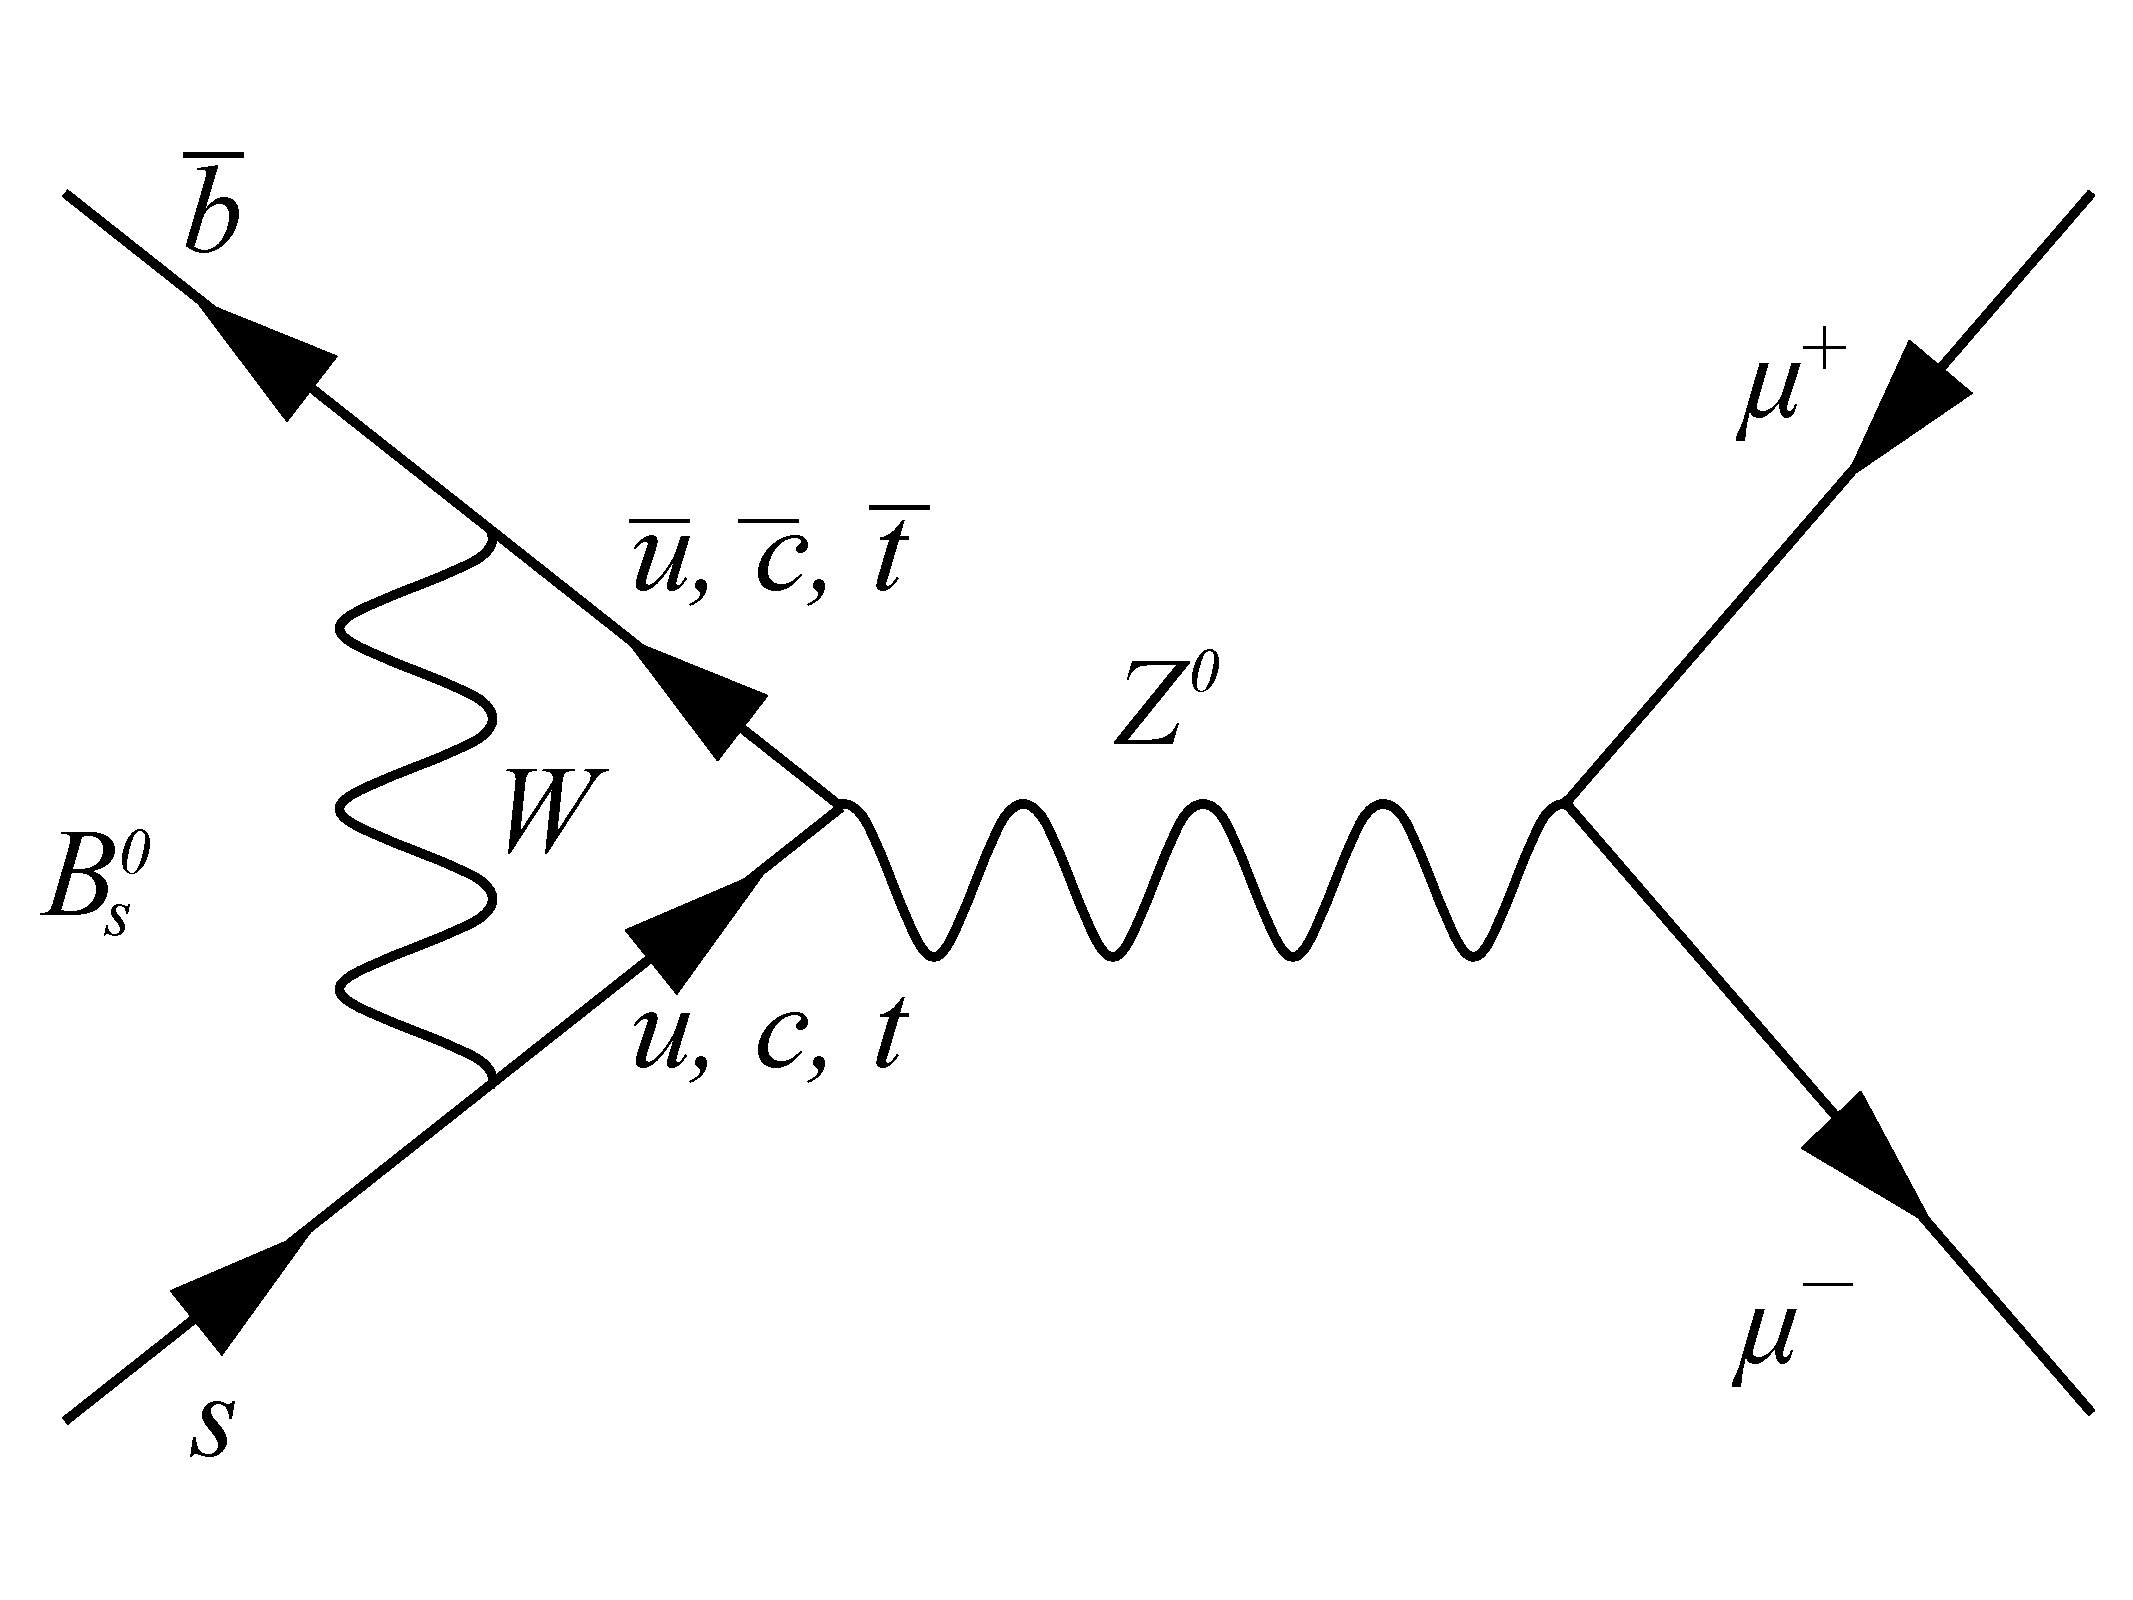
\includegraphics[width=0.4\textwidth]{./Figs/Theory/Z0_penguin_v2.pdf}
    \caption{Feynman diagrams for \bsmumu decays in the SM via $W$-box and $Z^0$-penguin processes. The same diagrams apply to \bdmumu decays where the $s$ quark is exchanged for a $d$ quark.}
    \label{fig:SM_diag}
\end{figure}

%The decays can also proceed via Higgs-penguin diagrams however the contributions from these diagrams are negligible~\cite{Arbey:2012ax}. %within the SM.                                                                                                                                   
%The lack of \bmumu decays at the tree level causes them to be suppressed compared to other \bsd decay modes that can occur at the tree level.

%The decays can also proceed via Higgs-penguin diagrams however the contributions from these diagrams are negligible. %within the SM.
%The lack of \bmumu decays at the tree level causes them to be suppressed compared to other \bsd decay modes that can occur at the tree level.

%{\it I think that this needs to be re-worded.

%Although the weak force allows quark flavour to change the coupling strengths between different quark flavours are not all the same magnitude. The coupling strengths are described by the CKM matrix. Quarks can Quarks fall into three families; $u$ and $d$, $c$ and $s$, $t$, and $b$. They can also be separated into two types depending on their charge; up-type quarks include $u$, $c$ and $t$, down-type quarks include $d$, $s$ and $b$. The weak force couples up-type quarks to the weak eigenstates of the down-type quark in the same family with the same strength. The weak quark eigenstates are not the same as the mass eigenstates and the two types of states are related via the CKM matrix as
%}

%{\it where $d^', s^'$ and $b^'$ are weak eigenstates and $d, s$ and $b$ are mass eigenstates. The CKM matrix is a unitary matrix, which ensures no tree level FCNCs occur, with complex elements that give the coupling strengths of different quarks, for example the amplitude of a $u$ quark changing into a $d$ quark is proportional to $|V_{ud}|$.}


Although the weak force allows quark flavour to change, the coupling strengths between different quark flavours are not all the same magnitude. This leads to the second source of suppression for \bmumu decays. The coupling strengths of different quarks are described by the Cabibbo-Kobayashi-Maskawa (CKM) matrix~\cite{PhysRevLett.10.531,doi:10.1143/PTP.49.652}. Quarks can be separated into two types depending on their charge: up-type quarks include $u$, $c$ and $t$; and down-type quarks include $d$, $s$ and $b$. The weak force couples all up-type quarks to the weak eigenstate of the down-type quark in the same family with the same strength, where the quark families are; $u$ and $d$, $c$ and $s$, $t$, and $b$. The weak quark eigenstates are not the same as the mass eigenstates and the two types of states are related via the CKM matrix as
\begin{equation}
\begin{pmatrix}
d'\\
s'\\
b'
\end{pmatrix}
= 
\mathbf{V_{CKM}}
\begin{pmatrix}
d\\
s\\
b
\end{pmatrix} =
 \begin{pmatrix}
   V_{ud} & V_{us} & V_{ub} \\
   V_{cd} & V_{cs} & V_{cb} \\
   V_{td} & V_{ts} & V_{tb}
 \end{pmatrix}
\begin{pmatrix}
d\\
s\\
b
\end{pmatrix},
\label{eq:CKMA}
\end{equation}
where $d'$, $s'$ and $b'$ are weak eigenstates and $d$, $s$ and $b$ are mass eigenstates. The CKM matrix is a unitary matrix with complex elements that ensure no tree level FCNCs occur. Each element of the matrix gives the coupling strengths of transitions between the mass eigenstates of quarks, for example the amplitude of a $u$ quark changing into a $d$ quark is proportional to $|V_{ud}|$.

The difference in the coupling strength sizes can be illustrated through the Wolfenstein parametrisation of the CKM matrix~\cite{PhysRevLett.51.1945}, which parametrises the matrix elements in powers of the small parameter of $\lambda = 0.22 \approx |V_{us}|$. The CKM matrix then becomes
\begin{equation}
\mathbf{V_{CKM}} =
 \begin{pmatrix}
 1 - \frac{1}{2}\lambda^2 & \lambda & \lambda^3 A (\rho - i \eta) \\
 - \lambda                & 1 - \frac{1}{2}\lambda^2 & \lambda^2 A \\
 \lambda^3 A (1 - \rho- i \eta) & -\lambda^2 A & 1
 \end{pmatrix} + \mathcal{O}(\lambda^4).
\label{eq:CKMB}
\end{equation}
This parametrisation shows that the CKM matrix is almost diagonal. For a \bmumu decay to occur, a single off-diagonal element is needed to describe the quark transitions in Figure~\ref{fig:SM_diag}, thus introducing an additional source of suppression to the decay. 
The internal quark lines in Figure~\ref{fig:SM_diag} can have contributions from $u$, $c$ and $t$ quarks. However, in the SM the contributions from $u$ and $c$ quarks are negligible when compared to the $t$ quark. This is due to the large $t$ quark mass compared to the other quarks, as given in Table~\ref{tab:fermions}, and because the coupling strength of the $b$ quark to any quark except the $t$ is extremely small due to additional powers of $\lambda$ in Equation~\ref{eq:CKMB}.


The final source of suppression of \bmumu decays comes from the helicities of the muons in the final state. Both \bd and \bs are spin zero particles and for angular momentum to be conserved in the decay the spins of the two muons must be oppositely aligned. This leads to the muons having opposite helicities. % Therefore the production of one of the muons will always be suppressed.
The weak force only couples to left-handed particle states and right-handed anti-particle states. In the high energy limit where particles are massless, negative helicity states are equal to left-handed states and positive helicity states are equal to right-handed states.
Therefore if the muons were massless the weak interaction could only produce a $\mu^-$ and a $\mu^+$ with opposite helicities which cannot conserve angular momentum in \bmumu decays.
Muons are not massless, therefore \bmumu decays can occur but are suppressed because $m_{\mu} \ll M_{B_{(s)}$~\cite{Olive:2016xmw}, leading to one of the helicity states of the muons always being disfavoured.

Overall \bmumu decays are highly suppressed within the framework of the SM compared to other decay modes of \bsd mesons. Therefore these decays offer excellent processes in which to search for NP because the contribution of BSM theories to these decay rates can be of a similar order of magnitude to those from the SM.

\section[\bmumu Branching Fraction]{\boldmath{\bmumu} Branching Fraction}
\label{sec:BFdef}
The \BF of a particle decay offers an excellent observable through which predictions of the SM can be compared to measured values. The \bmumu \BF is defined as the fraction of the total number of \bsd particles that decay into two muons. It can be calculated from the time-dependant decay rate, $\Gamma(B^0_{(s)}(t) \to \mu^+ \mu^-)$, which is the probability per unit of time that a \bsd decays into two muons, as
\begin{equation}
\mathcal{B}(B^0_{(s)} \to \mu^+ \mu^-) \equiv \frac{\Gamma(B^0_{(s)}(t) \to \mu^+ \mu^-) + \Gamma(\
\overline{B}^0_{(s)}(t) \to \mu^+ \mu^-)}{\Gamma(B^{0}_{(s)}) + \Gamma(\overline{B}^{0}_{(s)}) }.
\end{equation}
where $\Gamma(\overline{B}^0_{(s)}(t) \to \mu^+ \mu^-)$ is defined in an analogous way to $\Gamma(B^0_{(s)}(t) \to \mu^+ \mu^-)$, $\Gamma(B^0_{(s)})$ is the total decay rate for \bsd mesons and $\Gamma(\overline{B}^{0}_{(s)})$ is the total decay rate for $\overline{B}^0_{(s)}$ mesons. 
The SM predictions are calculated from the `prompt' decay rate which ignores any evolution with time of \bsd mesons. The \BFs are calculated using~\cite{DeBruyn:2012wj} 
\begin{equation}
\mathcal{B}(B^0_{(s)} \to \mu^+ \mu^-)_{\mathrm{th}} = \frac{ \tau_{B_{(s)}} }{2} \langle \Gamma(B^0_{(s)}(t) \to \mu^+ \mu^-) \rangle \big{|}_{t=0},
\label{sec:BF_prompt}
\end{equation}
where $\tau_{B_{(s)}$ is the mean lifetime of the \bsd and $\langle \Gamma(B^0_{(s)}(t) \to \mu^+ \mu^-) \rangle$ is the untagged decay rate, defined as
\begin{equation}
\langle \Gamma(B^0_{(s)}(t) \to \mu^+ \mu^-) \rangle = \Gamma(B^0_{(s)}(t) \to \mu^+ \mu^-) + \Gamma(\overline{B}^0_{(s)}(t) \to \mu^+ \mu^-).
\end{equation}
The untagged decay rate makes no distinction between the particle and anti-particle decays, and is accessible by experiments provided \bsd and $\overline{B}^{0}_{(s)}$ are produced in equal numbers. % this quantity is measured by experiments.
The \BFs are calculated this way to enable easy comparison of different $B$ meson \BFs including \bd, \bs and $B^+$~\cite{DeBruyn:2012wj}.

The prompt decay rate is evaluated from Fermi's golden rule, relating the transition amplitude, $\left|\mathcal{M}(B^0_{(s)} \to \mu^+ \mu^-)\right|$, and the kinematics of the decay to the decay rate as~\cite{Tolk:2148631}
\begin{equation}
\Gamma(B^0_{(s)}(t) \to \mu^+ \mu^-)\big{|}_{t=0} = \frac{1}{16\pi} \frac{1}{M_{B^0_{(s)}}} \sqrt{1 -4 \left (\frac{m_{\mu}}{M_{B^0_{(s)}}} \right )^2} \left|\mathcal{M}(B^0_{(s)} \to \mu^+ \mu^-)\right|^{2},
\label{sec:FGR}
\end{equation}
where $m_{\mu}$ and $M_{B^{0}_{(s)}}$ are the masses of the muon and the \bsd, respectively. %The factor $m_{\mu}/M_{B^{0}_{(s)}}$ is from the helicity suppression discussed in Section~\ref{sec:bsmumu_in_SM}.


Weak decays like \bmumu include interactions that occur at different energy scales, from the weak propagators at $M_W \approx 80$~\gevcc to the strong coupling in the \bsd meson at $\Lambda_{QCD} \sim 0.2$~\gev~\cite{Olive:2016xmw}. %This enable the Operator Product Expansion~\cite{} method to be used to construct the effective Hamiltonian, $\mathcal{H}_{eff}$, and calculate the transition amplitude $|\matcal{M}(B^0_{(s)} \to \mu^+ \mu^-)| = \langle \mu \mu | \mathcal{H}_{eff} | B^0_{(s)} \rangle$. The effective Hamiltonian divides the interaction into two energy levels with the structure
The Operator Product Expansion~\cite{PhysRev.179.1499,Wilson1972} is used to create the Effective Hamiltonian, $\mathcal{H}_{\mathrm{eff}}$, which splits the interaction into two very different energy levels. The transition amplitude then becomes 
\begin{equation}
|\matcal{M}(B^0_{(s)} \to \mu^+ \mu^-)| \equiv \langle \mu \mu | \mathcal{H}_{\mathrm{eff}} | B^0_{(s)} \rangle  = \frac{G_F}{\sqrt{2}} \displaystyle\sum_{i} V^i_{CKM} \langle \mu \mu | \mathcal{C}(\lambda)_i \mathcal{O}(\lambda)_i | B^0_{(s)} \rangle
\label{sec:eff_hamil_def}
\end{equation}
where $G_F$ is the Fermi coupling constant, $V_{CKM}^i$ are CKM matrix elements, $\matcal{C}_i$ are Wilson coefficients, $\mathcal{O}_i$ are local operators and $i$ is the sum over all possible Wilson coefficient and operator pairs. The energy scale $\lambda$ separates the two energy levels in the interaction. The Wilson coefficients describe short scale processes with energies above $\lambda$. This incorporates the internal structure and loops of Feynman diagrams leading to the dependence of Wilson coefficients on the $W^{\pm}$, $Z^0$, $H^0$ and $t$ quark masses. The long distance processes are described by the local operators $\mathcal{O}_i$ for energies less than $\lambda$. The local operators link the initial and final states of the decay. % indendant of the internal structure of the interaction. 
Wilson coefficients can be calculated using perturbation theory. However, this cannot be used for the local operators which can lead to large theoretical uncertainties on their values. The choice of $\lambda$ is arbitrary; however the final transition amplitude must be independent of $\lambda$. Often the mass of the decaying particle is used. 

%The Operator Product Expansion can be used to describe weak decays with different initial and final states as well as internal structure. 
In the Effective Hamiltonian in Equation~\ref{sec:eff_hamil_def} the CKM matrix elements are factored out of the Wilson coefficients and operators, so the same coefficients and operators can be used to describe both the \bd and \bs decays.
The Effective Hamiltonian for \bmumu decays is~\cite{DeBruyn:2012wk}
\begin{equation}
\mathcal{H}_{\mathrm{eff}} = -\frac{G_F \alpha}{\sqrt{2\pi}} V_{tq}^{*}V_{tb} \displaystyle\sum_{i}^{10,S,P} (\mathcal{C}_i\mathcal{O}_i + \matcal{C}^{'}_{i}\matcal{O}_{i}^{'}),
\label{eq:eff_hamil_bmumu}
\end{equation}
where $\alpha$ is the fine structure constant and $q$ corresponds to the $d$ quark in the \bd or the $s$ quark in the \bs. The terms proportional to $V^*_{cq}V_{cb}$ and $V^*_{cq}V_{ub}$ are negligible and can be neglected in Equation~\ref{eq:eff_hamil_bmumu}. The operators that can contribute to the \bmumu Effective Hamiltonian due to the initial and final decay states are
\begin{align}
 \mathcal{O}_{10}&=(\bar{q}\gamma^{\mu}P_{L}b)(\bar{l}\gamma_{\mu}\gamma_{5}l), &\qquad
 \mathcal{O}_{10}^{(')}&= (\bar{q}\gamma^{\mu}P_{R}b)(\bar{l}\gamma_{\mu}\gamma_{5}l), \\
 \mathcal{O}_{S}&= m_{b}(\bar{q}P_{R}b)(\bar{l}l),  &\qquad
\mathcal{O}_{S}^{(')}&= m_{b}(\bar{q}P_{L}b)(\bar{l}l), \\
 \mathcal{O}_{P}&= m_{b}(\bar{q}P_{R}b)(\bar{l}\gamma_{5}l), &\qquad
 \mathcal{O}_{P}^{(')}&= m_{b}(\bar{q}P_{L}b)(\bar{l}\gamma_{5}l).
\end{align}
%\begin{eqnarray}
% \mathcal{Q}_{10}&=(\bar{q}\gamma^{\mu}P_{L}b)(\bar{l}\gamma_{\mu}\gamma_{5}l),  \qquad
% \mathcal{Q}_{10}^{(')}&= (\bar{q}\gamma^{\mu}P_{R}b)(\bar{l}\gamma_{\mu}\gamma_{5}l), \\
% \mathcal{Q}_{S}&= m_{b}(\bar{q}P_{R}b)(\bar{l}l),  \qquad
%\mathcal{Q}_{S}^{(')}&= m_{b}(\bar{q}P_{L}b)(\bar{l}l), \\
% \mathcal{Q}_{P}&= m_{b}(\bar{q}P_{R}b)(\bar{l}\gamma_{5}l),  \qquad
% \mathcal{Q}_{P}^{(')}&= m_{b}(\bar{q}P_{L}b)(\bar{l}\gamma_{5}l) 
%\label{eq:operators}
%\end{eqnarray}
The operator $\mathcal{O}_{10}$ encompasses the only significant contributions in the SM that come from $W$-box and $Z^0$ penguin diagrams. The operator $\mathcal{O}_{10}^'$ describes the equivalent interactions as $\mathcal{O}_{10}$ but for right handed currents that are forbidden in the SM. %, de and $\mathcal{O}_{10}^'$ does not contribute in the SM because is describes right handed currents.% which are forbidden in weak interactions in the SM are described by $\mathcal{O}_{10}^'$ and 
 Finally, the operators $\mathcal{O}_{S}^{(')}$ and $\mathcal{O}_{P}^{(')}$ correspond to the exchange of scalar and pseudo-scalar particles which are negligible in the SM. 

The purely leptonic final state of \bmumu decays means that the computation of the transition amplitude can be spilt in two so that all uncertainties arising from the bound \bsd states are encompassed into one parameter, $F_{B_{(s)}}}$, the hadronic decay factor. This leads to a theoretically clean prediction for the \BF.

The \BFs for \bmumu decays can therefore be written as~\cite{Buras:2013uqa}
\begin{align}
\mathcal{B}(B^{0}_{(s)} \to \mu^{+} \mu^{-})=\frac{\tau_{B_{(s)}}G_{F}^{4} M_{W}^{4} \sin^{4}\theta_{W} }{8\pi^{5}} &\big|\mathcal{C}_{10}^{\mathrm{SM}} V^{*}_{tq}V_{tb}\big|^{2} F_{B_{(s)}}M_{B^0_{(s)}} m_{\mu}^{2} \nonumber \\ 
&\qquad {} \times \sqrt{1 - \frac{4m_{\mu}^{2}}{M^{2}_{B_{(s)}}}} (|P|^{2} + |S|^{2}),
\label{eq:BF_form}
\end{align}
where $\theta_W$ is the weak mixing angle and $M_{W}$ the mass of the $W$ boson. The \BF has been parametrised in terms of $\mathcal{C}_{10}^{\mathrm{SM}}$, $P$ and $S$, where $\mathcal{C}_{10}^{\mathrm{SM}}$ is the SM value of the operator $\mathcal{C}_{10}$ and 
\begin{equation}
P \equiv |P| e^{i\varphi_P} \equiv \frac{\mathcal{C}_{10} - \mathcal{C}_{10}^{'}}{\mathcal{C}_{10}^{\mathrm{SM}}} + \frac{M^2_{B^{0}_{(s)}}}{2m_{\mu}} \frac{m_b}{m_b + m_q} \frac{\mathcal{C}_{P} - \mathcal{C}_{P}^{'}}{\mathcal{C}_{10}^{\mathrm{SM}}},
\label{eq:P}
\end{equation}
and
\begin{equation}
S \equiv |S| e^{i\varphi_S} \equiv \sqrt{1- \frac{4m_{\mu}^{2}}{M^{2}_{B^{0}_{(s)}}}} \frac{M^{2}_{B^{0}_{(s)}}}{2m_{\mu}}  \frac{m_b}{m_b + m_q}  \frac{\mathcal{C}_{S} - \mathcal{C}_{S}^{'}}{\mathcal{C}_{10}^{\mathrm{SM}}}.
\label{eq:S}
\end{equation}
In the SM $P$ and $S$ are real, with the magnitudes $P=1$ and $S=0$, although the \BFs are parametrised in terms of $P$ and $S$ because BSM theories can significantly alter their values. 
%The dependence of the \BFs on $\mathcal{C}_{10}$ makes \bmumu decays one of the best decays to study this parameter and these decays are also very sensitive to scale particles~\cite{}. 
The presence of scalar particles could increase the \BFs above the SM expectation through $\mathcal{C}_S^{(')}$ leading to $S>0$. Furthermore, the contributions from scalar particles are not subject to helicity constraints. Additionally, pseudoscalar particles can either enhance or suppress the \BFs compared to the SM prediction depending on how the values of $\mathcal{C}_P^{(')}$ interfere with $\mathcal{C}_{10}^{(')}$ in NP models.


As well as the individual \BFs of \bdmumu and \bsmumu decays, the ratio of the two \BFs is also an interesting observable to test the flavour structure of the SM. 
%In the ratio the dependance on the Wilson coefficiencts cancels and the 
In the ratio the dependence of the \BFs on Wilson coefficients cancels, leaving it dependant on the elements $|V_{td}|$ and $|V_{ts}|$ of the CKM matrix. The ratio of \BFs is given by 
\begin{equation}
  \mathcal{R} \equiv \frac{\mathcal{B}(B^{0} \to \mu^{+} \mu^{-})}{\mathcal{B}(B^{0}_{s}\to \mu^{+} \mu^{-})} = \frac{\tau_{B}}{\tau_{B_{s}}}
 \bigg{|} \frac{V_{td}}{V_{ts}} \bigg{|}^{2} \frac{M_{B}^{2}}{M_{B_{s}}^{2}} \sqrt{\frac{1 - \frac{4m_{\mu}^{2}}{M^{2}_{B}}}{1- \frac{4m_{\mu}^{2}}{M^{2}_{B_{s}}}}}.
\label{eq:BF_ratio}
\end{equation}
Therefore the ratio provides a test of the coupling strengths of different quark types as described by the CKM matrix in the SM and could reveal whether or not BSM theories follow this structure as well. 
An additional advantage of using the ratio of \BFs is that the theoretical uncertainty on the ratio is less than the individual \BFs because sources of uncertainties including those from Wilson coefficients and $|V_{tb}|$ cancel.

%which probes the flavour structure of both the SM and BSM theories.
%The ratio does not depend on Wilson coefficients and thus provides an excellent observable to test the flavour structur\
%e of the SM and BSM theories. The ratio of \BFs is given by
%\begin{equation}
%  \mathcal{R} \equiv \frac{\mathcal{B}(B^{0} \to \mu^{+} \mu^{-})}{\mathcal{B}(B^{0}_{s}\to \mu^{+} \mu^{-})} = \frac{\tau_{B}}{\tau_{B_{s}}} \bigg{|} \frac{V_{td}}{V_{ts}} \bigg{|}^{2} \frac{M_{B}^{2}}{M_{B_{s}}^{2}} \sqrt{\frac{1 - \frac{4m_{\mu}^{2}}{M^{2}_{B}}}{1- \frac{4m_{\mu}^{2}}{M^{2}_{B_{s}}}}},
%\label{eq:BF_ratio}
%\end{equation}
%and the uncertainty on the ratio is less than the individual \BFs because sources of uncertainties including those from Wilson coefficients and $|V_{tb}|$ cancel. The ratio does not depend on Wilson coefficients and thus provides an excellent observable to test the flavour structure of the SM and BSM theories.


\section{Quark mixing}
\label{sec:quarkmaixing}
The theoretical prediction for the \bmumu \BFs described in Section~\ref{sec:BFdef} does not take into account the evolution of the \bsd and \barbsd mesons with time. Once a \bsd is created it will oscillate between the particle and anti-particle states as it propagates through time, the same is true for the \barbsd. Therefore the states that travel through time are a superposition of the \bsd and \barbsd. Oscillations occur as the constituent quarks transition between different flavours through the exchange of $W$ bosons as illustrated in Figure~\ref{fig:Oscl_diag}.
\begin{figure}[tbp]
    \centering
        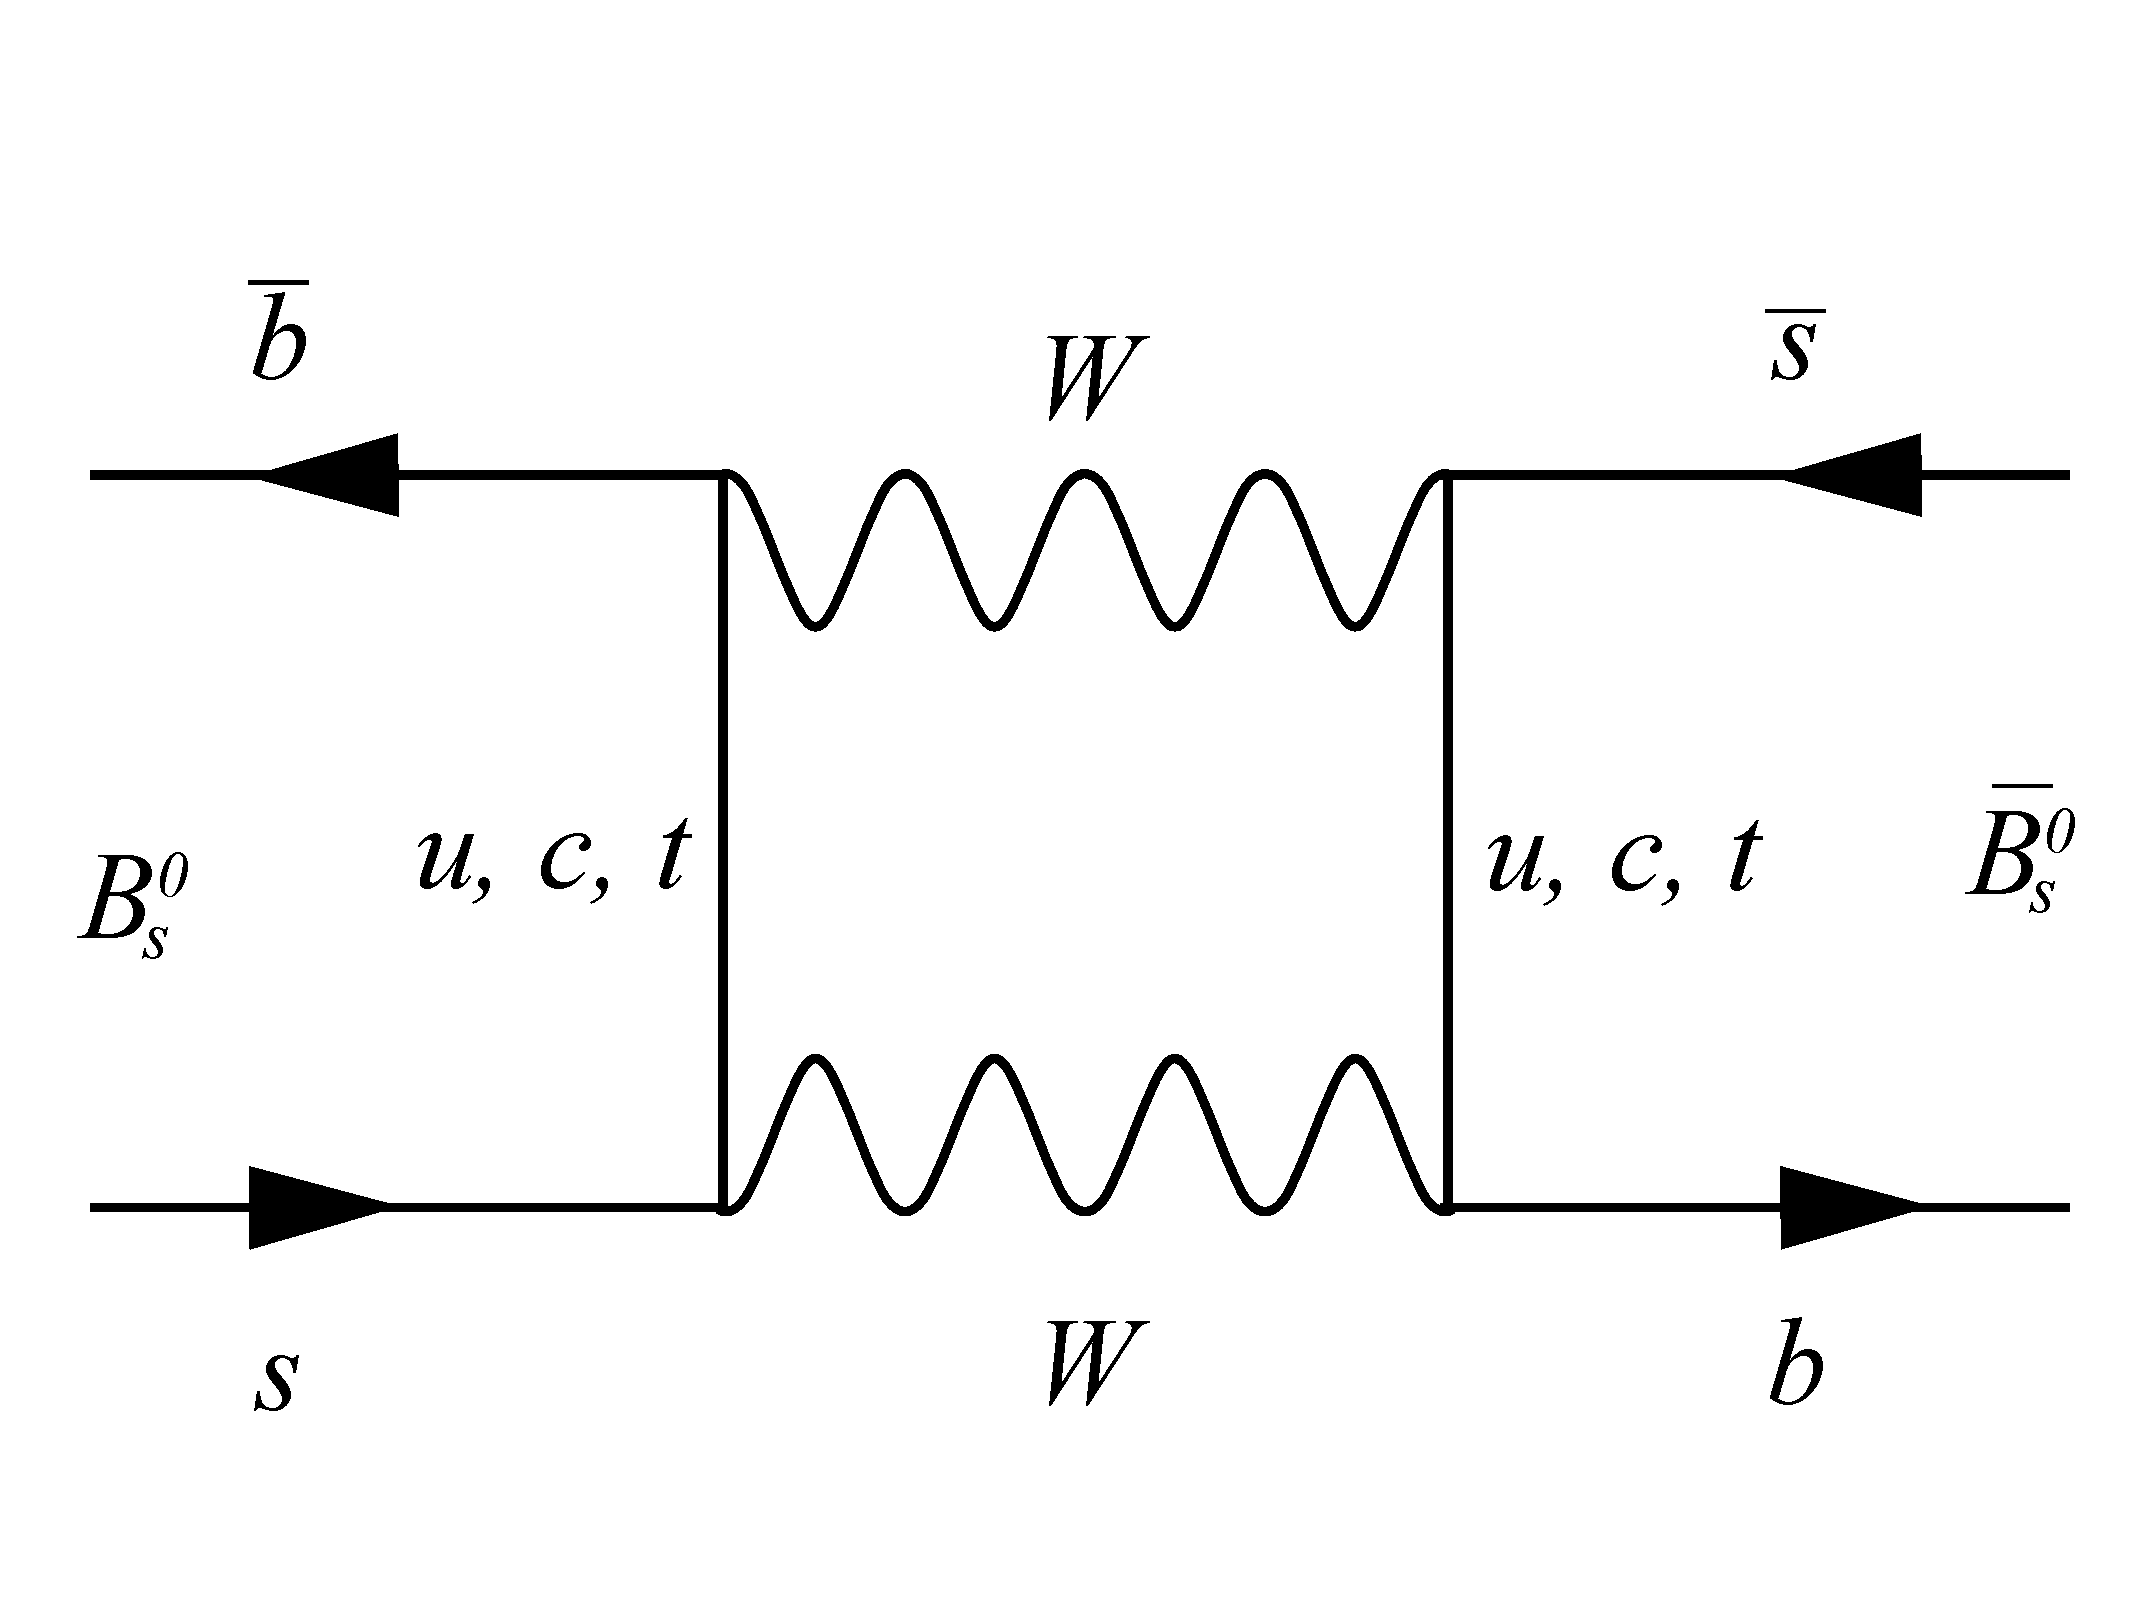
\includegraphics[width=0.6\textwidth]{./Figs/Theory/Oscillation_1.pdf}
        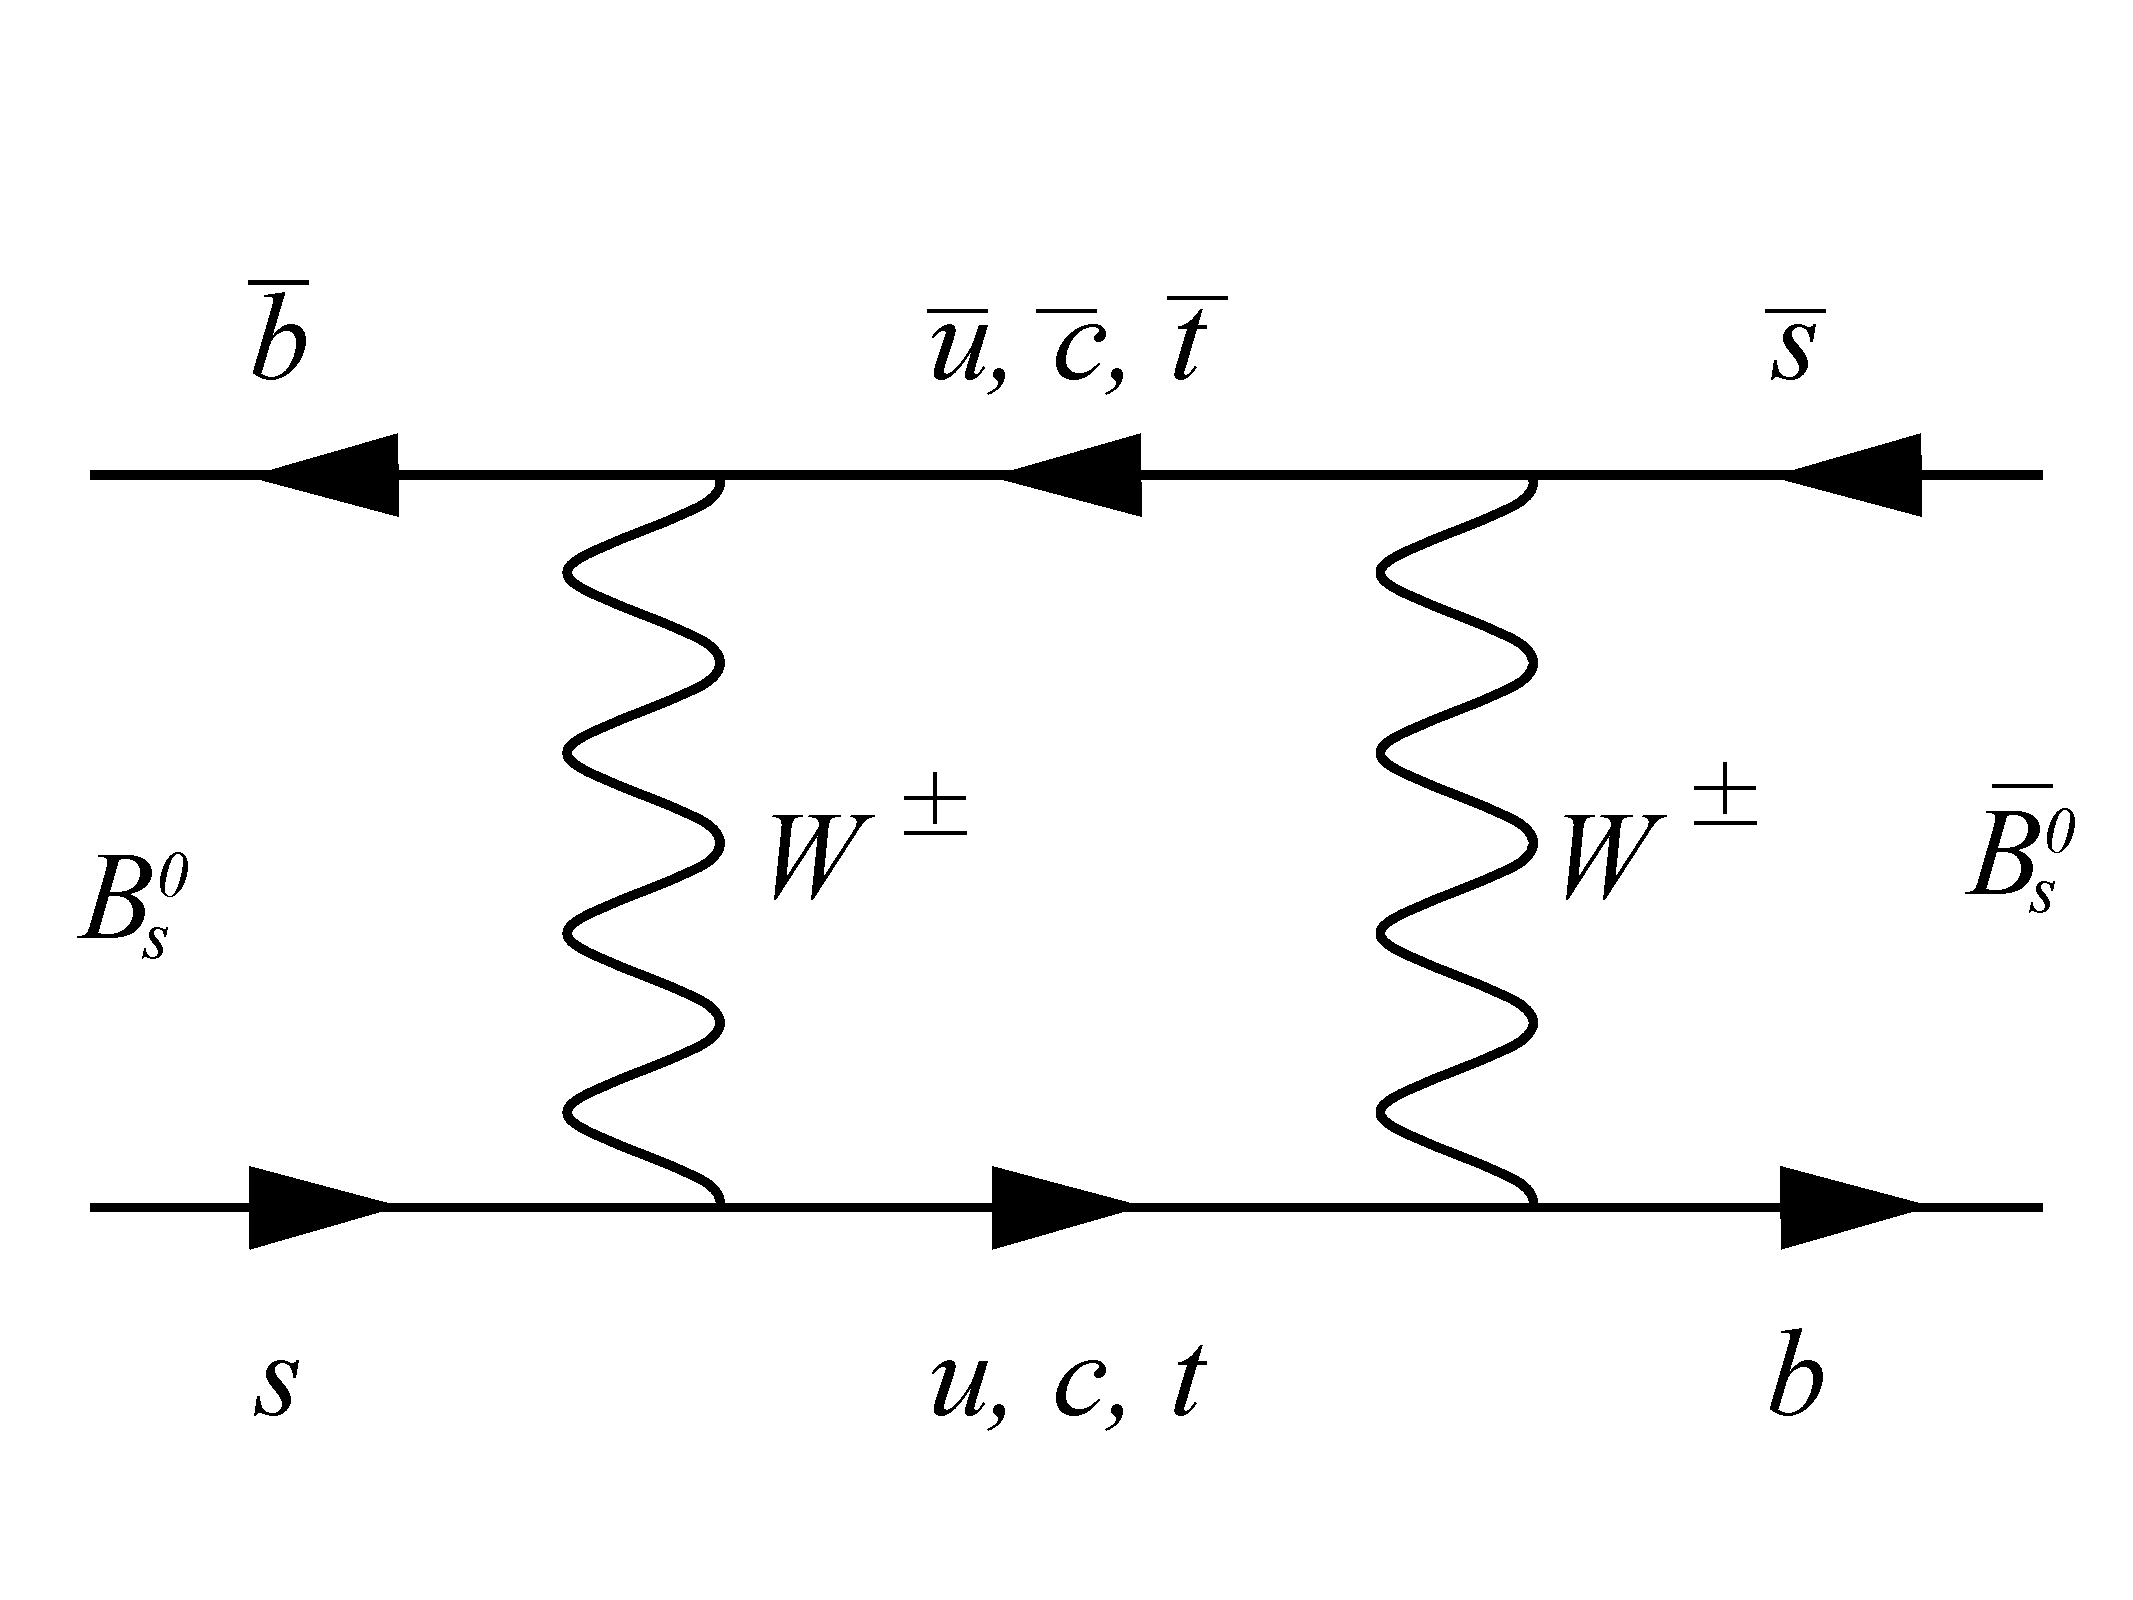
\includegraphics[width=0.6\textwidth]{./Figs/Theory/Oscillation_2.pdf}
    \caption{Oscillation of \bs and \barbs quarks through the exchange of $W$ bosons. The same diagrams apply to \bd and \barbd oscillations but with the $s$ quark exchanged for a $d$ quark.}
    \label{fig:Oscl_diag}
\end{figure}
The \BFs are measured from data where \bsd and \barbsd decays are not separated, which is called an untagged sample of \bmumu decays. Since a \bsd or \barbsd lives for $\sim10^{-12}$~s before decaying, the state that decays will not necessarily be the same as the one that was produced. The measured \BF is not the same as the `prompt' \BF used for the theoretical prediction. The measured value corresponds to the time integrated \BF given by~\cite{DeBruyn:2012wj}
\begin{equation}
  \mathcal{B}(B^0_{(s)} \to \mu^+ \mu^-)_{\mathrm{exp}} \equiv \frac{1}{2} \int^{\infty}_0 \langle \Gamma(B^0_{(s)}(t) \to \mu^+\mu^-) \rangle dt.
\label{eq:time_BF}
\end{equation}
Therefore for a meaningful comparison between the measured and predicted \BF values, the difference in the two definitions must be evaluated~\cite{DeBruyn:2012wj,DeBruyn:2012wk,Buras:2013uqa}. %,DeBruyn:2012wj}.

\subsection[Time evolution of the \bsd]{Time evolution of the \boldmath{\bsd}}
\label{sec:oscillations}
In $pp$ collisions, initially each $b$ and $\bar{b}$ quark hadronises to form a \bsd or \barbsd described at $t=0$ by the states $| B^0_{(s)} \rangle$ and $| \overline{B}^0_{(s)} \rangle$. The time evolution of these states must be evaluated in order to determine the time integrated \BFs. The Time-Dependent Schr\"{o}dinger Equation (TDSE) describes the time evolution of the particle and anti-particle states as
\begin{equation}
i \frac{d}{dt}\begin{pmatrix}{| B^0_{(s)}(t) \rangle \\ | \overline{B}^0_{(s)}(t) \rangle }\end{pmatrix} = \Bigg{(} \mathbf{M} - \frac{i\mathbf{\Gamma}}{2} \Bigg{)} \begin{pmatrix}{| B^0_{(s)}(t) \rangle \\ | \overline{B}^0_{(s)}(t) \rangle }\end{pmatrix}, 
\label{eq:TDSE}
\end{equation}
where $\mathbf{M}$ and $\mathbf{\Gamma}$ are $2 \times 2$ Hermitian matrices describing mass and decay time with the properties $M_{12}^{*} = M_{21}$ and $\Gamma_{12}^{*} = \Gamma_{21}$. Invariance under charge, parity and time inversion introduces additional constraints of $M_{11} = M_{22}$ and $\Gamma_{11} = \Gamma_{22}$. 

The \bsd-\barbsd oscillations ensure that for any $t>0$ the particles are a superposition of $| B^0_{(s)} \rangle$ and $| \overline{B}^0_{(s)} \rangle$ states. The off-diagonal elements in the mass and decay time matrices mean that the eigenstates of the TDSE have different masses and lifetime to the \bsd and \barbsd. The eigenstates can be defined at $t=0$ as
\begin{equation}
| B_H \rangle = p | B^0_{(s)} \rangle - q |\overline{B}^0_{(s)} \rangle, \qquad |B_L \rangle = p  | B^0_{(s)} \rangle + q | \overline{B}^0_{(s)} \rangle
\label{eq:mass_states}
\end{equation}
with eigenvalues of $(m_{H,L} - i\Gamma_{H,L}/2)$ and the coefficients $p$ and $q$ are constrained by $|p|^2 + |q|^2 = 1$. The eigenstates are known as heavy, $| B_H \rangle$, and light, $| B_L \rangle$, mass eigenstates. The eigenvalues are different for the \bd and \bs systems, however the treatment of the two systems is identical. To simplify the notation only the \bs system will be described in the following discussion.
The time evolution of the heavy and light mass eigenstates is given by
\begin{equation}
  | B_H (t)\rangle = | B_H \rangle e^{-i(m_H - i\frac{\Gamma_H}{2})t}, \qquad | B_L (t)\rangle = | B_L \rangle e^{-i(m_L - i\frac{\Gamma_L}{2})t}
\label{eq:time1}
\end{equation}
from the TDSE. Therefore, the time evolution of the flavour states can now be determined from Equations~\ref{eq:mass_states} and~\ref{eq:time1} as
\begin{align}
| B^{0}_{s}(t) \rangle &= \frac{1}{2p}\left(|B_{L}(t)\rangle + |B_{H}(t) \rangle \right)  = f_{+}(t) |B^{0}_{s} \rangle + \frac{q}{p}f_{-}(t) |\overline{B}^{0}_{s}\rangle  \label{eq:AAA}\\
| \overline{B}^{0}_{s}(t) \rangle &= \frac{1}{2q}\left(|B_{L}(t)\rangle - |B_{H}(t) \rangle \right)  = \frac{p}{q}f_{-}(t) |B^{0}_{s} \rangle+ f_{+}(t) |\overline{B}^{0}_{s}\rangle \label{eq:BBB}
\end{align}

%\begin{align}
%\left| B^{0}_{s}(t)} \right \rangle &= \frac{1}{2p}(| B_{L} (t)\rangle  + | B_{H{ (t)\rangle) \nonumber \\
%&= f_{+}(t) | B^{0}_{(s)} \rangle  + \frac{q}{p} f_{-}(t)\overline{B}^{0{_{(s)} \rangle \\
%\left| \overline{B}^{0}_{s}(t) \right\rangle &= \frac{1}{2q}(| B_{L} (t)\rangle -  | B_{H} (t)\rangle) \nonumber \\
%&= \frac{p}{q}f_{-}(t)| B^{0}_{s} \rangle  + f_{+}(t)\overline{B}^{0}_{s} \rangle 
%\end{align}
where 
\begin{equation}
f_{\pm} = \frac{1}{2} e^{-i(m_s - i\Gamma_s)t} \left \{ e^{i(\Delta m_s + i \Delat\Gamma_s)t/2} \pm e^{-i(\Delta m_s + i \Delat\Gamma_s)t/2} \right \}.
\end{equation}
The relationships
\begin{align}
m_s &\equiv \frac{m_H + m_L}{2}, &  \Delta m_s &\equiv m_H - m_L,\\
\Gamma_s &\equiv \frac{(\Gamma_H + \Gamma_L)}{2}, & \qquad \Delta \Gamma_s &\equiv \Gamma_L - \Gamma_H,
\label{eq:deltas}
\end{align}
have been used in the expressions of $|B^{0}_{s}(t)\rangle$ and $|\overline{B}^{0}_{s} (t) \rangle$. The difference $\Delta m_s$ is defined so that it is always positive whereas $\Delta\Gamma_s$ can take either sign. The time evolution is written in terms of these variables because $\Delta m_s$ and $\Delta\Gamma_s$ are measurable quantities.

Theoretical predictions can be calculated for $M_{12}$ and $\Gamma_{12}$ and it is therefore useful to express the measurable quantities in terms of these parameters. This is done by solving the characteristic equation of the TDSE, $|\mathbf{M} - i \mathbf{\Gamma}/2 - \lambda \mathbf{I}| = 0$, which has the solutions
\begin{equation}
\Delta m_{s}^2 - \frac{\Delta\Gamma_{s}^2}{4} = 4(|M_{12}|^2 - \frac{1}{4} |\Gamma_{12}|^2) 
\end{equation}
\begin{equation}
\Delta m_{s} \Delta \Gamma_{s} = 4 |\Gamma_{12}| |M_{12}| \cos \phi
\end{equation}
where $\phi \equiv \mathrm{arg}(-M_{12}/\Gamma_{12})$.

The observed relationships $\Delta \Gamma_{s} \ll \Delta m_{s}$ and $\Gamma_{12} \ll M_{12}$~\cite{Nierste:2009wg} are used to separate the expressions for $\Delta m_{s}$ and $\Delta \Gamma_{s}$ to give
\begin{equation}
\Delta m_{s} = 2 |M_{12}| \left( 1 + \mathcal{O}\left ( \left | \frac{\Gamma_{12}}{M_{12}} \right |^2 \right) \right) 
\end{equation}
and
\begin{equation}
\Delta \Gamma_{s} = 2|\Gamma_{12}|\cos \phi  \left(1 + \mathcal{O} \left ( \left | \frac{\Gamma_{12}}{M_{12}} \right |^2 \right ) \right).
\end{equation}
The values of $p$ and $q$ can also be related to the measurable quantities and $\Gamma_{12}$ and $M_{12}$ by diagonalising $(\mathbf{M} - \frac{i}{2}\mathbf{\Gamma})$ to produce
\begin{align}
\frac{q}{p} &= -\frac{\Delta m_{s}^{2} + i \Delta \Gamma_{s}/2 }{2M_{12} - i \Gamma_{12}} \approx - e^{-i\phi_{M}}\left (1-\frac{a}{2} \right ) + \mathcal{O}\left ( \left | \frac{\Gamma_{12}}{M_{12}} \right |^{2} \right ) 
\end{align}
where $\phi_M \equiv \mathrm{arg}(M_{12}/|M_{12}|)$ and $ a \equiv |\Gamma_{12}}/M_{12}|}\sin \phi$ and the relationships $\Delta \Gamma \ll \Delta m$ and $\Gamma_{12} \ll M_{12}$ have been used. The value of $\phi_M$ is related to the elements of the CKM matrix and $\phi_M = \mathrm{arg}(V_{tb}^*V_{td})$ for the \bd and $\phi_M = \mathrm{arg}(V_{tb}^*V_{ts})$ for the \bs. The ratio of $p$ and $q$ is given in terms of the small parameter $a$ which is needed to evaluate some SM processes but can be neglected in this process. 

The necessary parameters used to describe the time evolution of \bsd and \barbsd states have now been expressed in terms of measurable or predictable quantities, and therefore the time-dependant decay rates can now be evaluated. The decay rates can be expressed as
\begin{equation}
\Gamma (B^0_{(s)}(t) \to \mu^+ \mu^-) = \mathcal{N} \left|\mathcal{M}(B^0_{(s)} \to \mu^+ \mu^-)\right|^{2}
\end{equation}
and
\begin{equation}
 \Gamma (\overline{B}^0_{(s)}(t) \to \mu^+ \mu^-) =\mathcal{N}\left|\mathcal{M}(\overline{B}^0_{(s)} \to \mu^+ \mu^-)\right|^{2},
\label{eq:CCC}
\end{equation}
where $\mathcal{N}$ equals the additional terms in Equation~\ref{sec:FGR} from kinematic parameters and $\left|\mathcal{M}(B^0_{(s)} \to \mu^+ \mu^-)\right|$ and $\left|\mathcal{M}(\overline{B}^0_{(s)} \to \mu^+ \mu^-)\right|$ are the transition amplitudes for the particle and anti-particle decays as used in Equation~\ref{sec:FGR}. For the evaluation of the time-dependant decay rates, the exact form of the transition amplitudes are not needed. A new parameter is defined
\begin{equation}
\lambda_{\mu\mu} = \frac{q}{p} \left| \frac{\overline{A}_{\mu\mu}}{A_{\mu\mu}}\right|,
\end{equation}
where $A_{\mu\mu} = \mathcal{M}(B^0_{(s)} \to \mu^+ \mu^-)$ and $\overline{A}_{\mu\mu} = \mathcal{M}(\overline{B}^0_{(s)} \to \mu^+ \mu^-)$, to simplify the decay rate expression. Combining the information in Equations~\ref{eq:AAA}, \ref{eq:BBB} and \ref{eq:CCC}, ignoring terms of $\mathcal{O}(a)$ and using $\lambda_{\mu\mu}$ the time-dependant decay rates are
\begin{align}
\Gamma(B^0_s(t) \to \mu^+ \mu^-) &=  \frac{1}{2} \mathcal{N} |A_{\mu\mu}|^2 e^{- \Gamma_s t} \bigg\{ (1 + |\lambda_{\mu\mu}|^2) \cosh \left( \frac{\Delta \Gamma_s t}{2} \right) \nonumber \\
& \quad {}+ ( 1 - |\lambda_{\mu\mu}|^2) \cos(\Delta m_s t) - 2\mathrm{\Re}(\lambda_{\mu\mu})\sinh \left(\frac{\Delta \Gamma_s t}{2}\right)\nonumber \\
& \quad {} - 2\mathrm{\Im}(\lambda_{\mu\mu})\sin(\Delta m_s t) \bigg\} \label{eq:decayratesApart} 
\end{align}
and
\begin{align}
\Gamma(\overline{B}^0_s(t) \to \mu^+ \mu^-) &=  \frac{1}{2} \mathcal{N}|A_{\mu\mu}|^2 e^{- \Gamma_s t} \bigg\{ (1 + |\lambda_{\mu\mu}|^2) \cosh \left( \frac{\Delta \Gamma_s t}{2} \right) \nonumber \\
& \quad {}- ( 1 - |\lambda_{\mu\mu}|^2) \cos(\Delta m_s t) -2\mathrm{\Re}(\lambda_{\mu\mu})\sinh \left(\frac{\Delta \Gamma_s t}{2}\right) \nonumber\\ 
& \quad {}+ 2\mathrm{\Im}(\lambda_{\mu\mu})\sin(\Delta m_s t) \bigg\}. \label{eq:decayratesA}
\end{align}
The time integrated \BF depends on the sum of the \bsd and \barbsd time-dependant decay rates. Using Equation~\ref{eq:decayratesA}, the total decay rate is
\begin{equation}
\langle \Gamma (B^0_s(t) \to \mu^+ \mu^-) \rangle & = \mathcal{N} |A_{\mu\mu}|^2 (1 + |\lambda_{\mu\mu}|^2) e^{- \Gamma_s t} \left(\cosh \left( \frac{\Delta \Gamma_s t}{2} \right) + A_{\Delta\Gamma}\sinh \left(\frac{\Delta \Gamma_s t}{2}\right)\right). 
\label{sec:decayratesB}
\end{equation}
The parameter, $A_{\Delta \Gamma}$, has been introduced into the total decay rate and it is defined as
\begin{equation}
A_{\Delta\Gamma} = \frac{2\mathrm{\Re}(\lambda_{\mu\mu})}{1 + |\lambda_{\mu\mu}|^2} .
\label{eq:A_DGa}
\end{equation}
The meaning of $A_{\Delta\Gamma}$ can be seen when the total decay rate is written in terms of the heavy and light \bsd mass eigenstates as
\begin{align}
  \langle\Gamma (B^0_s(t) \to \mu^+ \mu^-) \rangle &= \mathcal{N} |A_{\mu\mu}|^2 (1 + |\lambda_{\mu\mu}|^2) \left( (1 - A_{\Delta\Gamma})e^{-\Gamma_L t} + (1 + A_{\Delta\Gamma})e^{-\Gamma_{H} t} \right) \nonumber \\
&= R_H e^{-\Gamma_H t} + R_L e^{-\Gamma_L t}.
\label{eq:decayratesC}
\end{align}
This final expression for the decay rates shows how \bmumu decays can be described in terms of the sum of the decays of the heavy and light mass eigenstates. The parameter \ADG is therefore related to the number of heavy and light mass eigenstates that decay as
\begin{equation}
A_{\Delta\Gamma} = \frac{R_H - R_L}{R_H + R_L}.
\end{equation}
The values \ADG can take range from +1 when only heavy mass eigenstates decay as \bsmumu and $-1$ when only light mass eigenstates decay as \bsmumu. The same is true for the \bdmumu decay.
\subsection{Impact on the Branching Fraction}
\label{sec:BFimpact}
The time-dependent decay rates are used to understand the difference between the two \BF definitions. The final form of the decay rates in Equation~\ref{eq:decayratesC} is used in the evaluation of the \BFs. The `prompt' \BF used in the theoretical predictions is
\begin{align}
\mathcal{B}(B^{0}_{(s)} \to \mu^{+} \mu^{-})_{\mathrm{th}} &= \frac{\tau_{B_{(s)}}}{2} \langle \Gamma(B^{0}_{(s)}(t) \to \mu^{+} \mu^{-}) \rangle \big{|}_{t=0}\\
&=\frac{\tau_{B_{(s)}}}{2} (R_{H} + R_{L}).
\end{align}
%\begin{align}
%  \mathcal{B}(B^{0}_{(s)} \to \mu^{+} \mu^{-})_{th}& &\equiv \frac{\tau_{B_{(s)}}}{2}\langle \Gamma (B^{0}_{(s)} \to \mu^{+}\mu^{-}) \rangle \bigg|_{t=0}\nonumber \\
% &= \frac{\tau_{B_{(s)}}{2} (R_{H} + R_{L})
%\end{align}
The time integrated \BF that is measured is
\begin{align}
  \mathcal{B}(B^{0}_{(s)} \to \mu^{+}\mu^{-})_{\mathrm{exp}} &= \frac{1}{2} \int^{\infty}_0 \langle \Gamma (B^{0}_{(s)} \to \mu^{+}\mu^{-}) \rangle  dt \nonumber \\
&= \frac{1}{2} \left( \frac{R_{H}}{\Gamma_{H}} + \frac{R_{L}}{\Gamma_{L}} \right) \nonumber \\
&= \frac{\tau_{B_{(s)}}}{2}(R_{H} + R_{L}) \left[ \frac{1 + A_{\Delta\Gamma}y_{(s)}}{1 - y_{(s)}^{2}} \right],
\end{align}
where $y_{(s)}$ relates the heavy and light mass eigenstate decay times as $y_{(s)} = \Delta \Gamma_{(s)} / 2\Gamma_{(s)}$. Therefore the measured and prompt \BF values are related as
\begin{equation}
  \mathcal{B}(B^0_{(s)} \to \mu^+\mu^-)_{\mathrm{exp}} = \left[ \frac{1 + A_{\Delta\Gamma}y_{(s)}}{1 - y_{(s)}^{2}} \right] \mathcal{B}(B^0_{(s)} \to \mu^+ \mu^-)_{\mathrm{th}}.
\end{equation}
For $B^0$-$\overline{B}^0$ oscillations the difference in the lifetimes of the heavy and light mass eigenstates is extremely small. Therefore $y$ is negligible and the prompt \BF is equivalent to the experimental \BF. However, for \bs-$\overline{B}^0_s$ oscillations there is a large difference in the lifetimes of the mass eigenstates and $y_s =0.065 \pm 0.005$~\cite{Olive:2016xmw}. The prompt \BF must therefore be corrected to account for the oscillations before it is compared to the experimental value.
\section[\ADG and the \bsmumu effective lifetime]{\boldmath{\ADG} and the \boldmaht{\bsmumu} effective lifetime}
\label{sec:ADG_EL}
The definition of \ADG in Equation~\ref{eq:A_DGa} shows that it depends upon the transition amplitude of \bsmumu decays. In Section~\ref{sec:BFdef} the Effective Hamiltonian for this decay was discussed and the \BF given in terms of the complex variables $P$ and $S$. Therefore \ADG can also be expressed in terms of these parameters as~\cite{DeBruyn:2012wk}
\begin{equation}
A_{\Delta \Gamma} = \frac{|P|\cos \varphi_P + |S| \cos \varphi_S}{|P|^2 + |S|^2},
\label{eq:NP_ADG}
\end{equation}
where $P$ and $S$ are defined in Equations~\ref{eq:P} and~\ref{eq:S}, respectively.
In the SM, $P=1$ and $S=0$, therefore \ADG takes the maximal value of +1 and only the heavy mass eigenstate decays as \bsmumu. This can be understood because the final state of a \bsmumu decay is a $\mathcal{CP}$ odd state and the heavy \bs mass eigenstate is a $\mathcal{CP}$ odd state.

As discussed in Section~\ref{sec:BFdef}, NP models can alter the values of $P$ and $S$, moving them away from the SM expectations. A change in these values could alter both the measured \BF and \ADG or just one of these observables. Since the comparison of the measured \BF to the SM prediction relies on \ADG, in order to understand possible NP contributions to the \BF, \ADG must be measured as well. 

The value of \ADG can be measured directly from the time-dependant decay rate of \bsmumu decays. This method involves separating the \bsmumu decays into those with $| B^0_s \rangle$ and $|\overline{B}^0_s\rangle$ initial states, which requires a large number of \bsmumu decays. Since \bsmumu are very rare decays this approach is currently not viable. Alternatively \ADG can be measured through the \bsmumu effective lifetime~\cite{DeBruyn:2012wj}. The effective lifetime is the mean decay time of an untagged sample of \bsmumu decays, defined as~\cite{Fleischer:2011cw}
\begin{equation}
  \tau_{\mu\mu} \equiv \frac{\int^{\infty}_0 t \langle \Gamma (B^0_s \to \mu^+ \mu^-) \rangle dt}{\int^{\infty}_0 \langle \Gamma (B^0_s \to\mu^+ \mu^-) \rangle dt}.
\label{eq:EL_def}
\end{equation}
%It can be measured by fitting a single exponential to the same set of decays used to measure the \BF~\cite{DeBruyn:2012wj}. 
It can be expressed in terms of \ADG using the decay rates in Equation~\ref{eq:decayratesC} as
\begin{align}
\tau_{\mu\mu} %&=\frac{\frac{R_{H}}{\Gamma_{H}^{2}} + \frac{R_{L}}{\Gamma_{L}^{2}}}{\frac{R_{H}}{\Gamma_{H}^{2}} + \frac{R_{L}}{\Gamma_{L}}}  \nonumber \\
= \frac{\tau_{B_{s}}}{1 - y_{s}^{2}} \left ( \frac{ 1 + 2A_{\Delta\Gamma}y_{s} + y_{s}^{2}}{1 + A_{\Delta\Gamma}y_{s}} \right).
\label{eq:lifetimedef}
\end{align}
%\begin{align}
%\tau_{\mu\mu} &= \frac{\frac{R_{H}}{\Gamma_{H}^{2}} + \frac{R_{L}}{\Gamma_{L}^{2}}}{\frac{R_{H}}{\Gamma_{H}} + \frac{R_{L}}{\Gamma_{L}}}\\
%&=  \frac{\tau_{B_{s}}}{(1 - y_{s}^{2}) \frac{(1 + 2 A_{\Delta\Gamma}y_{s} + y_{s}^{2})}{(1 + A_{\Delta\Gamma}y_{s})}
%\label{eq:EL_ADG}
%\end{align}
In the SM only the heavy \bs mass eigenstate decays as \bsmumu and the \el equals the lifetime of the heavy mass eigenstate, $\tau_{\mu\mu} = \tau_H = \frac{1}{\Gamma_H}$. The effective lifetime offers a measurement complementary to the \BFs to study the SM and NP models in \bsmumu decays due to the dependence of the \el on \ADG.

The \bsmumu \el can be measured by fitting a single exponential to the same set of decays used to measure the \BF~\cite{DeBruyn:2012wj}. The LHCb experiment has measured the effective lifetimes of several \bs decays in this way. These measurements include the \bskpi effective lifetime~\cite{Aaij:2014fia} in which equal proportions of the heavy and light \bs mass eigenstates contribute to the decay in the SM and the \bskk and $B^{0}_{s} \to D^{-}_{s} D^{+}_{s}$ effective lifetimes~\cite{Aaij:2014fia,Aaij:1463886, Aaij:2013bvd} where only the light \bs mass eigenstate decays into the $K^{+}K^{-}$ and $D^{-}_{s} D^{+}_{s}$ final states in the SM. 
Also, the effective lifetimes of $B^{0}_{s} \to J/\psi f_{0}(980)$~\cite{Aaij:2012nta} and $B^{0}_{s} \to J/\psi K^{0}_{S}$~\cite{Aaij:2013eia} decays have been measured, both decays occur predominately via the decay of the heavy \bs mass eigenstate in the SM. All the measured effective lifetimes are consitent with the predictions of the SM. %The measurements listed here all rely on vairables that are correlated with the \bs decay time in order to identify the decay modes, the resulting selection removes a greater proportion of \bs decays with short lifetimes compared to those with longer lifetimes. The selection efficiency as a function of the decay time is accounted for in the measurement. However the \bskk effective lifetime has also been measured using a selection strategy that has a uniform selection efficency across differet decay times and the results . 


%the identification of these \bs decays in data relies on variables that are correlated with the \bs decay time and the resulting selection removes a greater proportion of \bs decays with short lifetimes compared to those with longer lifetimes. %However the \bskk effective lifetime has also been measured using a selection strategy that has a uniform selection efficiency across differet decay times. 


%proceeds via decays of equal proportions of heavy and light \bs mass eigenstates. 


% decays from the heavy and light \bs mass eigentstates
\section{The Standard Model predictions}
\label{sec:SM_predictions}

The SM provides precise predictions of the time-integrated \bmumu \BFs~\cite{Bobeth:2013uxa} %~\cite{Bobeth:2013uxa, Aoki:2016frl, Fleischer:2017ltw}
\begin{align}
\mathcal{B}(B^0_{s} \to \mu^+ \mu^-)& = (3.65 \pm 0.23) \times 10^{-9}\\
\mathcal{B}(B^0 \to\mu^+ \mu^-)& = (1.06 \pm 0.09) \times 10^{-10}
\end{align}
where the latest progress in lattice QCD calculations have been taken into account~\cite{Bazavov:2011aa, Na:2012kp,Witzel:2013sla}. % quark oscillations have been accounted for in the quoted valu~\cite{Bobeth:2013uxa, Aoki:2016frl, Fleischer:2017ltw}. 
The largest contributions to the theoretical uncertainties come from the CKM matrix elements and the decay constants of the \bs and the \bd.
The ratio of the \BF values, defined in Equation~\ref{eq:BF_ratio} is~\cite{CMS:2014xfa} 
\begin{equation}
\mathcal{R} = \frac{\mathcal{B}(B^0 \to\mu^+ \mu^-)}{\mathcal{B}(B^0_{s} \to \mu^+ \mu^-)} = 0.0295^{+0.0028}_{-0.0025}.
\end{equation}


The \bsmumu effective lifetime is determined from Equation~\ref{eq:lifetimedef}. Using the SM value of \ADG = +1, the \bs mean lifetime of $\tau_{B_{s}} = 1.505 \pm 0.005$~ps~\cite{Amhis:2016xyh} and $y_{s} = 0.065 \pm 0.005$~\cite{Olive:2016xmw} the SM effective lifetime is
%In the SM the \bsmumu effective lifetime is predicted to be~\cite{Fleischer:2017ltw}
\begin{equation}
\tau_{\mu\mu} = 1.609 \pm 0.010 \mathrm{ps},
\end{equation}
which is equal to the lifetime of the heavy \bs mass eigenstate as, in the SM, only the heavy mass eigenstate of the \bs decays into two muons. The same calculation can be performed for \ADG = $-$1, giving the lifetime of the light mass \bs eigenstate as $\tau_{L} = 1.413 \pm 0.006$~ps.
%The Heavy Flavour Averaging Group provides the world averages for the measured values of the lifetime of the light and heavy \bs mass eigenstates to be $\tau_{H} = 1.609 \pm 0.010$~ps and $\tau_{L} = 1.414 \pm 0.006$~ps~\cite{Amhis:2016xyh}.
The difference in these lifetimes is $0.195$~ps and therefore a precision of 0.38~ps would be needed to distinguish between \ADG~=~$+1$ and \ADG~=~$-1$ at 5$\sigma$ with the \el. 



\section[New Physics models and \bmumu decays]{New Physics models and \boldmath{\bmumu} decays}
\label{sec:NPmodels}
There exist a large number of BSM theories that can influence \bmumu decays in different ways. Measurements of the \bmumu \BFs and the \bsmumu effective lifetime can constrain the parameter space available for NP and in doing so could reveal which theories are viable extensions of the SM. This section will briefly introduce some NP models that could influence \bmumu decays given the current precision of the \BF measurements. %can be studied with \bmumu decays.
For more detailed discussions of NP models relevant to \bmumu decays and constraints on these models from measurements see references~\cite{Buras:2013uqa,Knegjens:2014zva,Altmannshofer:2014rta}.

As discussed in Section~\ref{sec:BFdef}, the ratio of the \bdmumu and \bsmumu branching fractions provides an excellent test of the flavour structure of the SM and BSM theories. %Both the measured ratio and theoretical predictions are more precise than the individual \BFs due to the cancellation of uncertainties in the ratio. 
Figure~\ref{fig:ratio} shows possible values accessible by BSM theories alongside the SM prediction. The prediction of the Minimal Flavour Violation (MFV)~\cite{DAmbrosio:2002vsn} hypothesis is included. % in Figure~\ref{fig:ratio}. 
\begin{figure}[tbp]
    \centering
        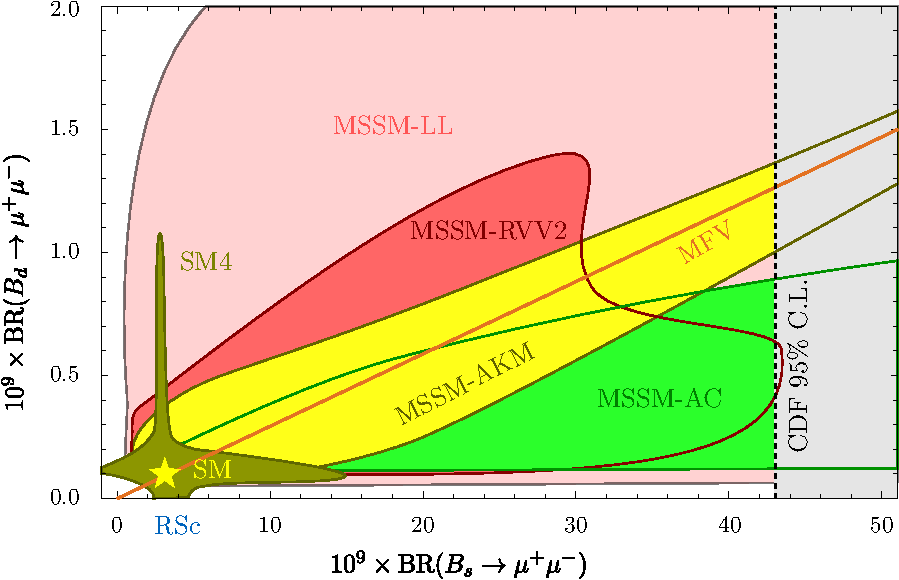
\includegraphics[width=0.8\textwidth]{./Figs/Theory/MFV.pdf}
    \caption{Correlations between the \bdmumu and \bsmumu \BFs including the SM prediction, the Minimal Flavour Violation hypothesis (MFV), four Minimal Supersymmetric Standard Models (MSSM)~\cite{Martin:1997ns} and the SM extended to contain four generations of fermions~(SM4)~\cite{Hou:2008xd}. Figure is taken from reference~\cite{Straub:2010ih}.}
    \label{fig:ratio}
\end{figure}
The MFV hypothesis predicts that the coupling of quark flavour and $\mathcal{CP}$ violation follow the same Yukawa structure as the SM in NP models. It is a popular theory to describe the flavour structure in NP models due to the current agreement of measurements with the SM predictions. A significant deviation of the \BF ratio from the SM or MFV hypothesis predictions would indicate the need for a new flavour structure in theoretical models.

Additionally, NP models could move the \BFs and \ADG away from the SM predictions by providing new particles that could contribute to the decays either through loop diagrams, similar to those in Figure~\ref{fig:SM_diag}, or allowing the decays to occur at the tree level. These new particles would change the Wilson coefficients included in the parameters $P$ and $S$. The dependence of the \BFs and \ADG on $P$ and $S$ are different, as shown in Equations~\ref{eq:BF_form} and~\ref{eq:NP_ADG}, and therefore NP models can influence the observables independently. The allowed values of \ADG and the ratio of the measured \BF to prompt SM prediction for \bsmumu decays are shown in Figure~\ref{fig:NPmodelsB} for possible situations where $S=0$, $P=1$, $P\pm S = 1$ and $\varphi_P, \varphi_S \in \{0, \pi\}$. These figures illustrate that if NP effects are not revealed in the \BF measurements, they could still appear in \ADG. 

\begin{figure}
  \centering
  \begin{subfigure}[b]{0.48\textwidth}
  \centering

    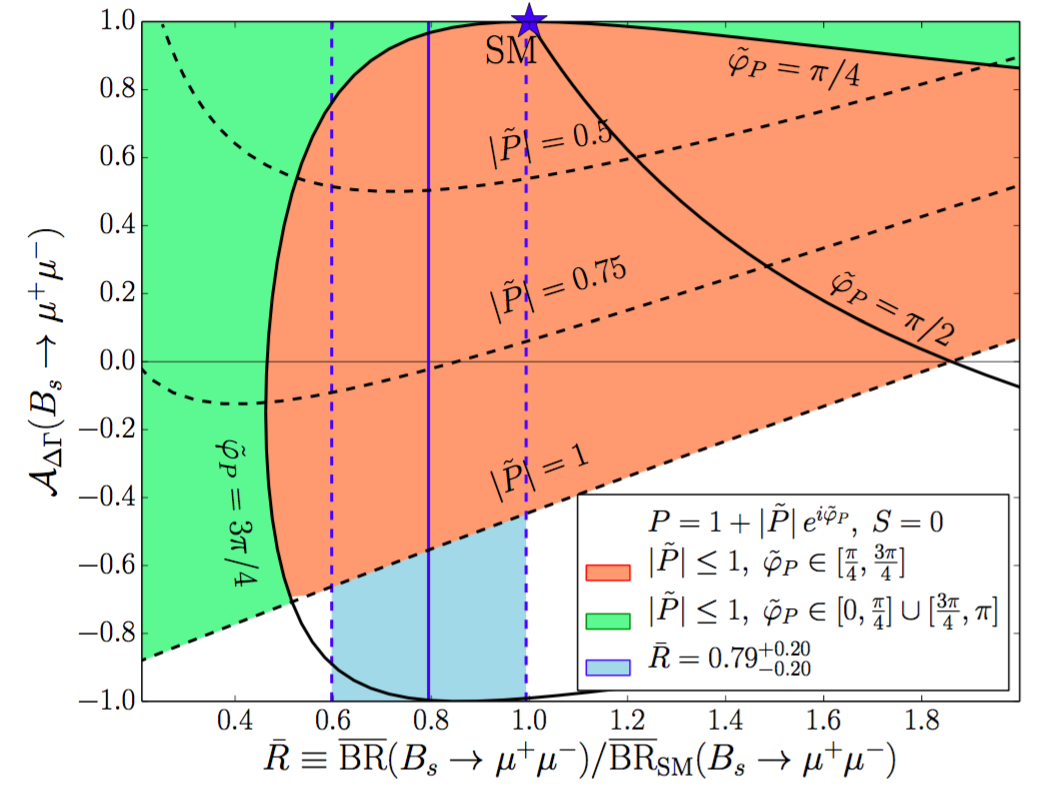
\includegraphics[width=\textwidth]{./Figs/Theory/NP_S_0.png}
    \caption{}
    \label{fig:TomJerry}   
  \end{subfigure}             
  \begin{subfigure}[b]{0.48\textwidth}
  \centering

    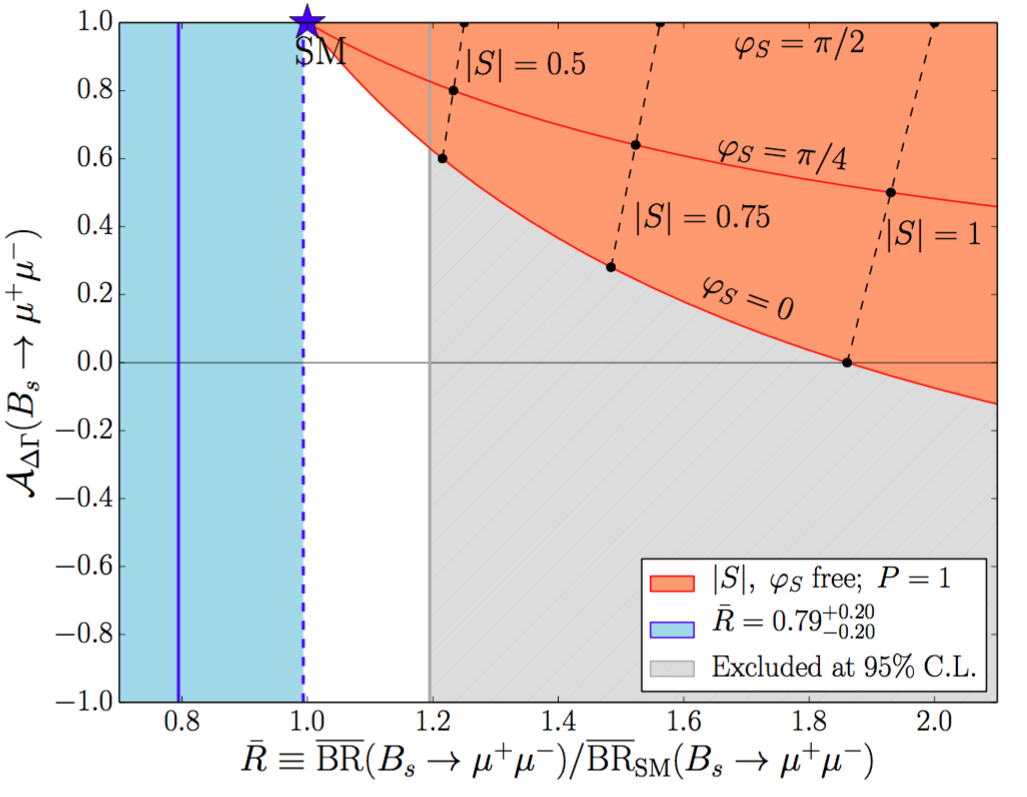
\includegraphics[width=\textwidth]{./Figs/Theory/NP_P_1.png}
    \caption{}
    \label{fig:WallE}
  \end{subfigure}             
  \begin{subfigure}[b]{0.48\textwidth}
  \centering

    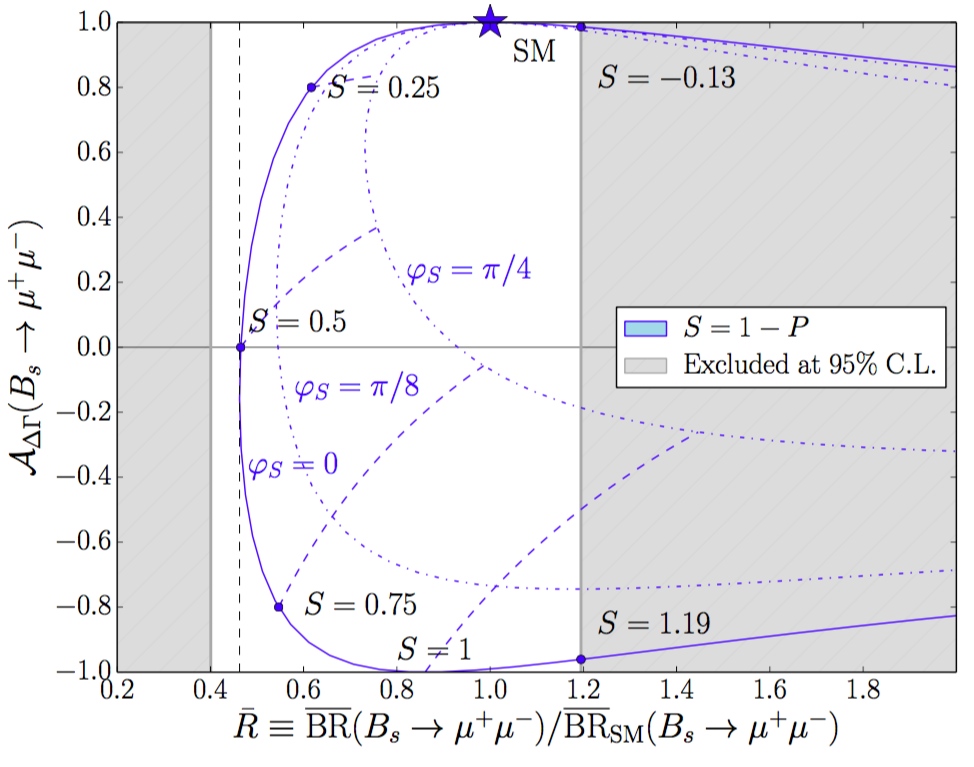
\includegraphics[width=\textwidth]{./Figs/Theory/NP_P_pm_S_1.png}
    \caption{}
    \label{fig:Minnion}
  \end{subfigure}
  \begin{subfigure}[b]{0.48\textwidth}
  \centering

    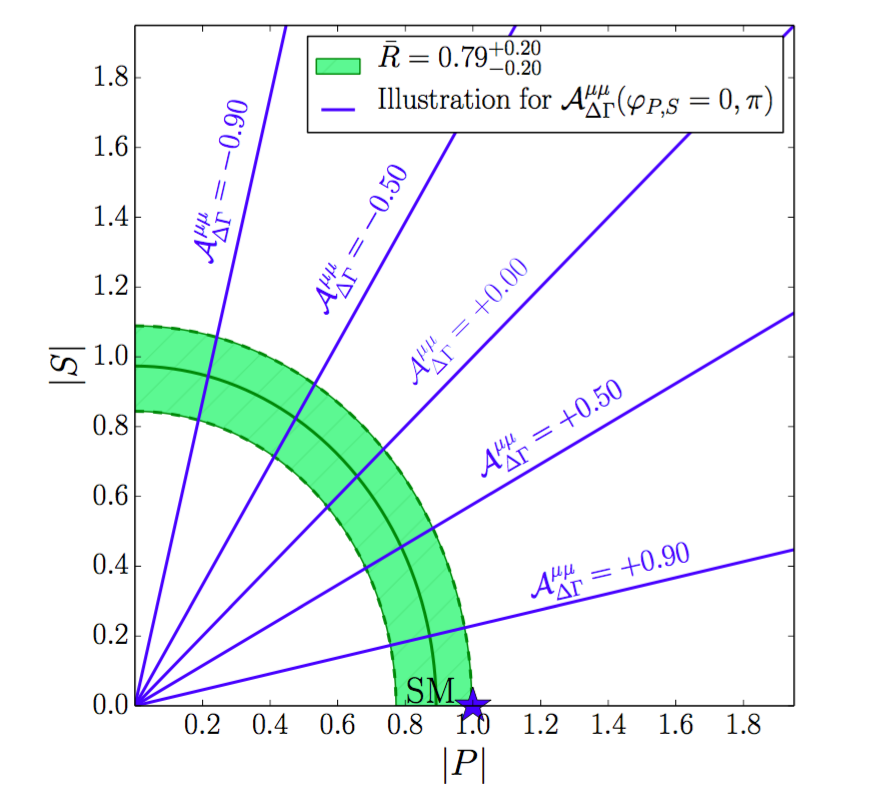
\includegraphics[width=0.9\textwidth]{./Figs/Theory/NP_phi.png}
    \caption{}
    \label{fig:Minn}
  \end{subfigure}
  \caption{Allowed values for $\mathcal{B}$(\bsmumu) and \ADG for situations where a) $S=0$, b) $P=1$, c) $P \pm S = 1$ and d) $\varphi_P, \varphi_S \in \{0, \pi\}$ (d)~\cite{Buras:2013uqa,Knegjens:2014zva}. The ratio $\overline{R}$ plotted is from an average of the individual results from the CMS and LHCb collaborations from~\cite{CMSandLHCbCollaborations:2013pla}, and the results from the combined analysis of the CMS and LHCb data gives $\overline{R} = 0.76^{+0.20}_{-0.18}$~\cite{CMS:2014xfa}.}
  \label{fig:NPmodelsB}
\end{figure}




Amongst the BSM theories that can influence the values of $P$ and $S$ are the Two Higgs Doublet Model (2HDM)~\cite{HALL1981397}, supersymmetric models~\cite{Witten:1981nf} and models including leptoquarks. % and models that obey the MFV hypothesis as mentioned earlier.

The 2HDM extends the Higgs sector of the SM by introducing two complex scalar field doublets both with non-zero vacuum expectation values. Spontaneous symmetry breaking then produces two charged, one neutral pseudoscalar and two neutral scalar Higgs bosons. The new particles can enter the loops of \bmumu decays and allow FCNCs to occur at the tree level. Different scenarios of this model depend on the Higgs-quark interactions and can incorporate the MFV hypothesis. This model can produce scenarios where $S=0$, $P=1$ or $P\pm S = 1$~\cite{Buras:2013uqa,Knegjens:2014zva} and the corresponding \BF and \ADG values for \bsmumu decays as shown in Figures~\ref{fig:TomJerry},~\ref{fig:WallE} and~\ref{fig:Minnion}.

Supersymmetric (SUSY) models extend the SM by giving each SM particle a supersymmetric partner. The resulting theory is symmetric in terms of the transformation of fermions to bosons and bosons to fermions. So far no evidence for SUSY particles has been found, and therefore the symmetry must be broken and the mass of SUSY particles are greater than their SM partners. The Minimal Supersymmetric Standard Model (MSSM) includes a Higgs sector similar to the 2HDM and there are scenarios where it obeys the MFV hypothesis. \bmumu decays are sensitive to this model provided the ratio of the vacuum expectation values of the Higgs doublet is large~\cite{Buras:2002wq,Babu:1999hn,Isidori:2001fv}. The MSSM can produce values for \ADG and the \bsmumu \BF shown in Figure~\ref{fig:Minnion} and~\ref{fig:Minn} for situations where $P\pm S =1$ and $\varphi_P, \varphi_S \in \{0, \pi\}$~\cite{Buras:2013uqa,Knegjens:2014zva}.

Models including leptoquarks are currently popular to explain the anomalies observed in heavy flavour measurements~\cite{Barbieri:2016las,Becirevic:2016yqi,Hiller:2014yaa,Bauer:2015knc,Fajfer:2015ycq}. A leptoquark is a boson that carries both lepton and baryons numbers, therefore leptoquarks can allow FCNCs to occur at the tree level. The exact quantum numbers of these particles depend on their interactions with SM fermions. Therefore leptoquarks could enhance \bmumu decays but information from \ADG is necessary for the study of leptoquarks with \bmumu decays because it resolves degeneracies that are present when only the \BF measurements are considered~\cite{Altmannshofer:2017wqy}.

Although \bmumu decays are yet to reveal NP, the current experimental precision still leaves plenty of room for NP to be revealed. The observation of \bsmumu decays makes it possible to start investigating \ADG through the \bsmumu \el. A measurement of \ADG will provide important information, complementary to the \bmumu \BF measurements in the search for NP in \bsmumu decays.


%Now let us reference some stuff. The old~\ref{fig:FD_ratioKPi} and the new~\ref{fig:Minnion}.
